\documentclass[12pt,a4paper,epsf,portrait,times,epsfig]{article}
%\usepackage[dvips]{graphics}
\usepackage{graphicx}
\usepackage{epsfig}
\usepackage{amsmath}
\usepackage{xspace}
\usepackage{fancybox}
\usepackage{rotating}
\usepackage{subcaption}
\usepackage{comment}
\usepackage{float}
\usepackage{upgreek}
\usepackage[utf8]{inputenc}
\usepackage[sort&compress, numbers, comma]{natbib}

\usepackage{color}
\usepackage{hyperref}
\hypersetup{
	colorlinks=true,
	linktoc=all,
	linkcolor=blue,
	citecolor=blue,
	urlcolor=blue,
}

\setlength{\parskip}{0.2cm}
\setlength{\parindent}{0.0cm}
\setlength{\textheight}{8.5in}
\setlength{\textwidth}{16.0cm}
\setlength{\oddsidemargin}{0in}
\setlength{\evensidemargin}{0in}
\setlength{\topmargin}{0in}
\raggedright

\usepackage{chngcntr}

\counterwithin{figure}{section}
\counterwithin{table}{section}

\DeclareUnicodeCharacter{0227}{a}

\begin{document}
	\begin{center}
		{\Large \bf Measurement of the associated production of a Z boson and bottom or charm quarks with the ATLAS experiment}
	\end{center}
		
		\vspace{3.0cm}
		
	\begin{center}
		{\Large \bf Jacob Oliver}
	\end{center}

		\vspace{1.5cm}
		
	\begin{center}
		\today
	\end{center}
		
		\vspace{3.0cm}
		
		
	\begin{center}
		{\large \bf Abstract}
	\end{center}
	This document presents the first step in obtaining unfolded cross sections of the Z$\rightarrow$($\ell\ell$)+b and Z$\rightarrow$($\ell\ell$)+bb channels with $\ell\ell$ corresponding to a muon or electron pair, in addition to measurements of kinematic variables. The analysis uses data collected by the ATLAS experiment at the LHC of p-p collisions corresponding to 139fb$^{-1}$ at a centre of mass energy of $\sqrt{s}$ = 13 TeV. The benefits of a measurement of unfolded cross sections of kinematic variables for these processes are briefly discussed before the presentation of the measurement results. The plots show a good modelling of data by the Monte Carlo simulation, and provide an adequate starting point for later analysis and unfolding of these cross sections.   
	
	\newpage
	\pagenumbering{roman}
	\tableofcontents
	\newpage
	\pagenumbering{arabic}
	
	\section{Introduction}
	
	The production of a Z boson from p-p collisions is an ideal target for analysis due to the strong identifiers of the process. The clear experimental signature of a Z boson decaying to a lepton pair is combined with the long lifetimes of b-hadrons to create a signature which is easy to observe, and that provides an excellent opportunity to study the production and dynamics of heavy flavour physics (heavy flavour physics is physics pertaining to quarks at the heavier end of the scale, namely bottom and charm, but not top quarks which have their own area of study). \par
	
	In the Standard Model (SM), there are multiple processes which create the signal source of Z boson production in association with two b quarks, with the Z boson later decaying to two leptons. While these processes occur via different mechanisms, they all arrive at the same final state which this analysis examines. The Z boson production is only possible through the electroweak interaction, however strong interactions also take place in each of the signal processes. The most common of the these processes occurs via the radiation of a gluon which splits into a bb pair. This is one of the central motivations to measuring Z$\rightarrow$($\ell\ell$)+bb processes: performing a measurement of the strong signal processes allows the investigation of QCD phenomena and strong coupling coefficients, which could potentially lead to a more precise SM in the future. \par
	
	Current Z$\rightarrow$($\ell\ell$)+bb cross sections are calculated using next-to-leading-order perturbative quantum chromodynamics (NLO pQCD), and are associated with large theoretical uncertainties \cite{Article:EarlyQCDCrossSections}. Cross sections of Z$\rightarrow$($\ell\ell$)+bb interactions have been available for some time \cite{Article:HeavyFlavourXsec1, Article:HeavyFlavourXsec2, Article:HeavyFlavourXsec3}. These processes have already been measured at lower centre of mass energy by both ATLAS \cite{Article:EarlyATLASCrossSecMeasurement}
	and CMS \cite{Article:EarlyCMSCrossSecMeasurement}, however performing a more current analysis allows for several improvements over previous studies. Key among these improvements is access to the full dataset produced by ATLAS during Run2, which allows the analysis to be extended to phase spaces with lower cross sections. \par
	
	\begin{comment}
	Currently NLO pQCD calculations involving heavy flavour are associated with one of two schemes named the four-flavour number scheme (4FNS) and five-flavour number scheme (5FNS). In the 4FNS b quarks appear only in the final state of a given process, and are considered to be massive (i.e. only the parton densities of gluons and the first two quark generations are considered within the proton). In the 5FNS, the presence of an additional b quark density is allowed within the initial state \cite{Article:PDG}. \par
	\end{comment}
	
	Currently NLO pQCD calculation involving heavy flavour are associated with one of two schemes named the four-flavour number scheme (4FNS) and five-flavour number scheme (5FNS). In the 4FNS b quarks do not contribute to the proton wave-function and are considered to be massive (i.e. only the parton densities of gluons and the first two quark generations are considered within the proton). In the 5FNS, the b quark is treated as massless and the presence of an additional b quark density is assumed within the proton \cite{Article:PDG}. \par
	
	By definition these schemes must always give identical results if contributions from all orders are added, however the manner of ordering the perturbative expansion is not consistent between the two schemes at any given order. This allows the possibility of a difference between the two schemes to arise, however this can only occur when the schemes are considered at a fixed order. There are advantages and disadvantages to each of the schemes \cite{Article:FlavourSchemes}, and this analysis allows an insight into both the 4FNS and 5FNS. \par
	
	\begin{comment}
	The Z$\rightarrow$($\ell\ell$)+bb process can be described by the 4FNS scheme as there are multiple mechanisms which allow for the production of a b quark pair in the final state, whereas the Z$\rightarrow$($\ell\ell$)+b process is described by the 5FNS scheme in order for an individual b quark to be present in the final state. As such, the Z$\rightarrow$($\ell\ell$)+b process allows for a b-quark density in the initial state. It is possible for quark-antiquark pairs with short lifetimes to be produced within the protons of the Large Hadron Collider (LHC) as quantum fluctuations from gluons. The quarks produced in these fluctuations are referred to as sea-quarks, and can interact with other present partons when the protons collide. \par
	\end{comment}
	
	The Z$\rightarrow$($\ell\ell$)+b process is a useful tool for probing the structure of the proton, due to the presence of the additional b quark density in the initial state of the proton prior to collision (as described by the 5FNS). The Z$\rightarrow$($\ell\ell$)+b is sensitive to this b quark density and measurements of its production could constrain the b quark parton density function (PDF)\cite{Article:PDFRun2} of the proton.
	
	Another benefit of performing a measurement of this process comes when considering its relation to other physical processes. The final state of a lepton pair and two b quarks is not	uncommon, and many other processes have similar final states which leads to Z$\rightarrow$($\ell\ell$)+bb being a common background. Many processes across multiple physical areas share this background, such as Higgs processes, and Dark Matter and SUSY searches. By obtaining a detailed measurement of Z$\rightarrow$($\ell\ell$)+bb production, it is possible to improve the precision
	of many searches with similar final states. \par

	There are, however, difficulties in performing a measurement such as this. Just as Z$\rightarrow$($\ell\ell$)+bb provides a background for many physical searches due to the shared final state, there are many additional background processes to Z$\rightarrow$($\ell\ell$)+bb. This makes a direct measurement difficult; an informed understanding of the background processes involved is essential in order to perform a good measurement. \par

	The following report outlines and explains the steps used to perform a measurement of these processes using data collected by ATLAS at the LHC.

	\newpage
	
	\section{Physical Theory}
	
	\subsection{The Standard Model}

	\begin{figure}[h!]
		\centering
		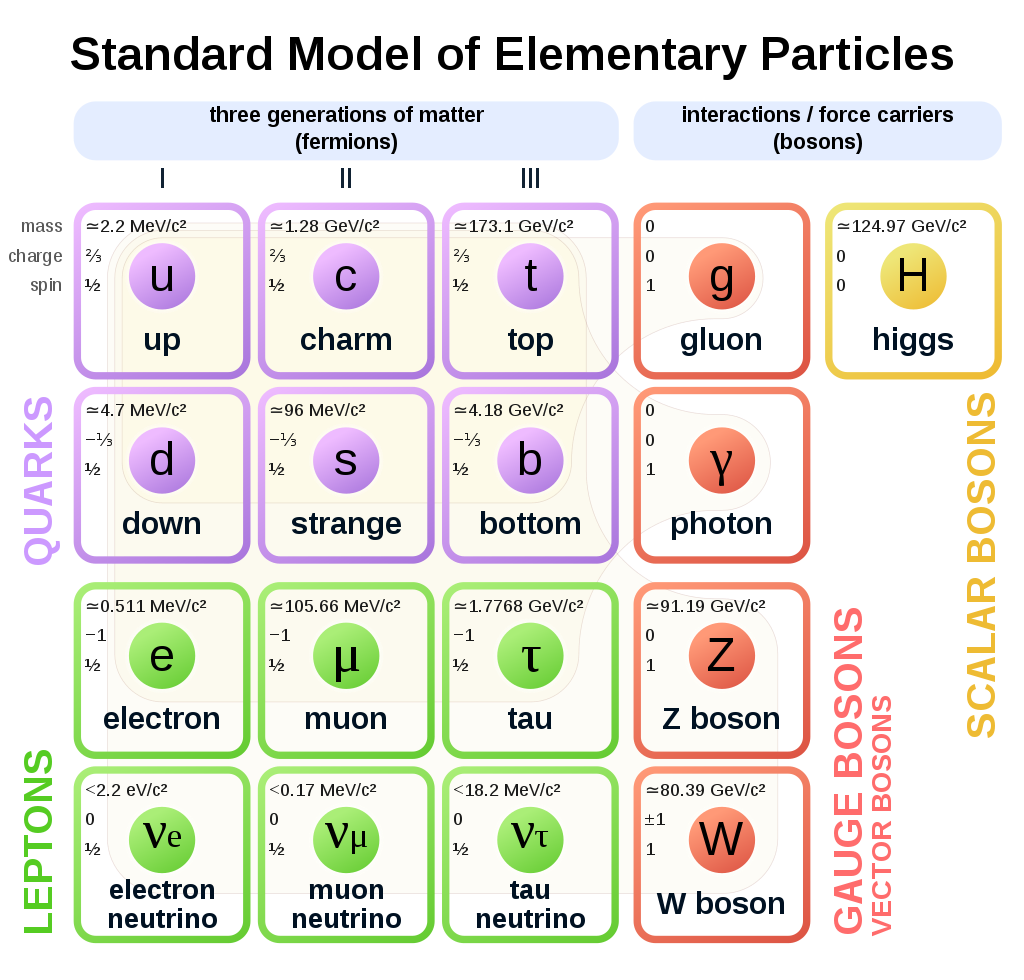
\includegraphics[scale=0.3]{Standard_Model.png}
		\caption{The Standard Model of particle physics.}
		\label{Fig:StandardModel} 
	\end{figure}

To study particle physics is to study the fundamental constituents of matter, and the interactions between them. In order to describe both these constituents and the interactions between them, a model called the Standard Model (SM) is used. The SM is a local, Lorentz-invariant quantum field theory. These interactions arise from the requirement of local gauge invariance within the SM, and can be described by group theory. The SM gauge group is as follows: 

\begin{center}
	\begin{equation}
	SU(3)_{C} \otimes SU(2)_{L} \otimes U(1)_{Y}
	\end{equation}
\end{center}

where $C$ is colour, $L$ is left-handedness, and $Y$ is hypercharge. 
In the SM, constituent matter particles are titled \textit{fermions}: half integer spin particles that obey Fermi Dirac statistics. The forces that cause the interactions between fermions are described by \textit{gauge bosons}: integer spin particles that obey Bose Einstein statistics. Each force is carried by a particular type of these mediator bosons: photons ($\gamma$) carry the electromagnetic force, gluons (g) carry the strong force, and W$^{\pm}$ and Z$^{0}$ bosons carry the weak force. Gravity is the only known fundamental force that is not described by the SM. Table \ref{tab:SMBosons} summarises the properties of the SM bosons. \par

\begin{table}
	\begin{center}
		\begin{tabular}{ |c|c|c|c|c|c| }
			\hline \hline
			Gauge Boson & Mass & Charge & Spin & Force & Theory \\
			\hline
			gluon & 0 & 0 & 1 & strong & QCD \\
			\hline
			W$^{\pm}$ & 80.379 $\pm$ 0.012 & $\pm$1 & 1 & weak & Electroweak \\
			\hline
			Z$^{0}$ & 91.1876 $\pm$ 0.0021 & 0 & 1 & weak & Electroweak \\
			\hline
			$\gamma$ & $ < 1 \times 10^{-18}$ & 0 & 1 & electromagnetic & Electroweak \\
			\hline \hline
		\end{tabular}
		\caption{A table showing the properties of the Standard Model gauge bosons\cite{Article:PDG}.}
		\label{tab:SMBosons}
	\end{center}
\end{table}

Fermions can be further subsectioned into two separate groups: quarks and leptons. Each group has three generations which, as a general rule of thumb, have increasing particle mass from generation to generation. \par

Leptons are classified by their charge ($Q$), lepton flavour number (the lepton flavour number is different for each generation of lepton and can be electron number (L$_{e}$), muon number (L$_{\mu}$), or tau number (L$_{\tau}$)), and the third component of weak isospin ($T_{3}$). It is also important to consider the additional quantity of weak hypercharge ($Y_{W}$) which is directly related to both the lepton charge and weak isospin by the equation:

\begin{center}
	\begin{equation}
	Y_{W} = 2\cdot(Q-T_{3})
	\end{equation}
\end{center}

The charged leptons (i.e. $e$, $\mu$, and $\tau$) are able to interact via both the weak and the electromagnetic force, however the neutral leptons ($\nu_{e}$, $\nu_{\mu}$, and $\nu_{\tau}$) can only interact with the weak force. Table \ref{tab:SMLeptons} summarises the properties of leptons within the SM. 

\begin{table}
	\begin{center}
		\begin{tabular}{ |c|c|c|c|c|c|c| }
			\hline \hline
			Lepton Flavour & Mass & Q & Y$_{W}$ & L$_{e}$ & L${\mu}$ & L$_{\tau}$ \\
			\hline
			e$^{-}$ & 0.511 MeV & -1 & -1 & 1 & 0 & 0 \\
			\hline
			$\nu_{e}$ & $<$ 2 eV & 0 & -1 & 1 & 0 & 0 \\
			\hline
			$\mu$ & 105.7 MeV & -1 & -1 & 0 & 1 & 0 \\
			\hline
			$\nu_{\mu}$ & $<$ 0.19 MeV & 0 & -1 & 0 & 1 & 0 \\
			\hline
			$\tau$ & 1776.8 MeV & -1 & -1 & 0 & 0 & 1 \\
			\hline
			$\nu_{\tau}$ & $<$ 18.2 MeV & -1 & -1 & 0 & 0 & 1 \\
			\hline \hline
		\end{tabular}
		\caption{A table showing the properties of the Standard Model leptons\cite{Article:PDG}.}
		\label{tab:SMLeptons}
	\end{center}
\end{table}

For each lepton a left-handed weak isospin doublet is formed:

\begin{equation}
	\begin{pmatrix}
		T_{3} = +1/2  \\
		T_{3} = -1/2  \\
	\end{pmatrix}=\begin{pmatrix}
		\nu_{eL} \\
		e_{L}^{-} \\
	\end{pmatrix},\begin{pmatrix}
		\nu_{\mu L} \\
		\mu_{L}^{-} \\
	\end{pmatrix},\begin{pmatrix}
		\nu_{\tau L} \\
		\tau_{L}^{-} \\
	\end{pmatrix}
\end{equation}

The SM forbids right-handed neutrinos, and as such weak isospin singlets (T$_{3}$ = 0) are formed by the right handed leptons in each generation: $e^{-}_{R}$, $\mu^{-}_{R}$, and $\tau^{-}_{R}$. 

Quarks are classified by their charge ($Q$), and their flavour quantum numbers: baryon number (the third component of the isospin ($I_{3}$)), strangeness ($S$), charmness ($C$), bottomness ($B$), and topness ($T$). Unlike the SM bosons and leptons, quarks are able to interact via all three of the fundamental forces. In addition to these flavour quantum numbers, quarks also have an additional quantum number named colour charge which can take one of three values (often referred to as red, blue, or green). The term colour only describes this quantum numbers, and not the colour of visible light. Table \ref{tab:SMQuarks} summarises the properties of the SM quarks.  


\begin{table}
	\begin{center}
		\begin{tabular}{ |c|c|c|c|c|c|c|c| }
			\hline \hline
			Quark Flavour & Mass & $Q$ & $I_{3}$ & $C$ & $S$ & $T$ & $B$ \\
			\hline
			u & 2.3$_{-0.5}^{+0.7}$ MeV & 2/3 & 1/2 & 0 & 0 & 0 & 0 \\
			\hline
			d & 4.8$_{-0.3}^{+0.7}$ MeV & -1/3 & -1/2 & 0 & 0 & 0 & 0 \\
			\hline
			c & 1.275 $\pm$ 0.025 GeV & 2/3 & 0 & 1 & 0 & 0 & 0 \\
			\hline
			s & 95 $\pm$ 5 MeV & -1/3 & 0 & 0 & -1 & 0 & 0 \\
			\hline
			t & 173.2 $\pm$ 0.9 GeV & 2/3 & 0 & 0 & 0 & 1 & 0 \\
			\hline 
			b & 4.18 $\pm 0.03$ GeV & -1/3 & 0& 0 & 0 & 0 & -1 \\
			\hline \hline
		\end{tabular}
			\caption{A table showing the properties and quantum numbers of the SM quarks\cite{Article:PDG}.}
			\label{tab:SMQuarks}
	\end{center}
\end{table}

In addition to the quarks and leptons, each fermion has its own antiparticle. These antiparticles are opposites to their matter particles, with reversed signs for all quantum numbers. We can obtain the total number of fermions in the standard model by simply summing their number: 6 leptons, 6 anti-leptons, 18 quarks (there are three variations for each quark flavour due to the three colour charges), and 18 antiquarks. This gives the SM a total of 12 leptons and 36 quarks. \par

The SM is a highly successful model and the predictions of the models have been tested to very high levels of accuracy by CERN, however it is known that the model is imperfect (hence the need for experimental physics). In order to improve the model, it must be rigorously tested in every facet until it is broken (such that it can then be revised and improved). \par

An example of this process can be seen by considering the constraint placed on the SM by electroweak (EW) theory: under EW theory, the masses of the W$^{\pm}$ and Z$^{0}$ bosons (i.e. the gauge bosons of the weak force) violate invariance under local gauge transformations. However, despite this the W$^{\pm}$ and Z$^{0}$ bosons have large masses. In order to account for this within the SM, the Higgs mechanism is required. The Higgs mechanism results in the presence of an additional gauge boson with a mass of 125 GeV in the SM known as the Higgs boson \cite{DiscoHiggsATLAS}\cite{DiscoHiggsCMS}. The Higgs mechanism is described in greater detail in section 2.2.3. \par

		\subsection{Describing the Standard Model Mathematically}
		
		\subsubsection{Quantum Chromodynamics}
		
		The strong interaction is described by a process known as Quantum Chromodynamics (QCD)\cite{Article:PDG}\cite{Article:QCDPrimer}: a non-Abelian gauge theory based on the SU(3) symmetry group of colour. This group has eight generators which correspond to the eight massless gluons that mediate the interactions of coloured quarks. These quarks are described by colour triplets:
		
		\begin{center}
			\begin{equation}
				q_{f}^{T} = (q_{f}^{1},q_{f}^{2},q_{f}^{3})
			\end{equation}
		\end{center}
	
		with 1, 2, and 3 representing the three colour states of red, green, and blue. 
		The Lagrangian density of QCD is given by
		
		\begin{center}
			\begin{equation}
				L_{QCD}=\sum_{j=1}^{n_{f}}\overline{q}_{j}(iD_{\mu}\gamma^{\mu}-m_{j})q_{j}-\frac{1}{4}\sum_{A=1}^{8}F^{A_{\mu\nu}}F_{\mu\nu}^{A}
			\end{equation}
		\end{center}
		
		The first sum of this equation corresponds to the quark contribution, and the second the gluon contribution. This equation is written with the quark-field spinors, $q_{j}$, and the quark masses $m_{j}$. $D_{\mu} = \partial_{\mu}-ig_{s}T_{A}\mathcal{A}_{\mu}^{A}$ is the covariant derivative, where $\mathcal{A}_{\mu}^{A}$ correspond to the gluon fields and $T_{A}$ to the eight generators of the SU(3) symmetry group. The $\gamma^{\mu}$ represent the Dirac matrices and $F_{\mu\nu}^{A}$ represents the field strength tensor based on the gluon field $\mathcal{A}_{\mu}^{A}$
		
		\begin{center}
			\begin{equation}
				F_{\mu\nu}^{A} = \partial_{\mu}\mathcal{A}_{\nu}^{A}-\partial_{\nu}\mathcal{A}_{\mu}^{A}-g_{s}f_{ABC}\mathcal{A}_{\mu}^{B}\mathcal{A}_{\nu}^{C}
			\end{equation}
		\end{center}
		
		with the QCD coupling constant, $g_{s} = \sqrt{4\pi\alpha_{s}}$, and the structure constants of the SU(3) symmetry group. \par 
		The SU(3) group is a non-Abelian group and as such the third term in Eq. 6 does not vanish and thus the present gluon fields are able to self-interact. The self interaction leads to asymptotic freedom as the effective coupling constant of the strong interaction decreases with increasing energy. In this case, quarks and gluons can be treated as free and their interactions can be calculated within perturbative theory. This is only allowed at short distance (equivalent to high energy), where the strong coupling constant converges asymptotically against zero. However, with increasing distance between two quarks (i.e. decreasing energy), the quarks become bounded in hadrons through a process called confinement.
		
		\subsubsection{Electroweak Theory} 
		
		The full gauge group of the SM gauge theory is SU(3)$\otimes$SU(2)$\otimes$U(1). Just as the non-Abelian group SU(3) gives rise to QCD, the non-Abelian group SU(2) and Abelian group U(1) give rise to the electroweak (EW) theory: the gauge theory behind the electroweak force. The electromagnetic and weak interactions can be unified under the SU(2)$\otimes$U(1) symmetry group, and this is described by EW theory. The SU(2) group involves three gauge fields with a corresponding gauge bosons of $W_{\mu}^{i}$ with $i = 1, 2, 3$. The U(1) group involves a single gauge field and a corresponding gauge boson of $B_{\mu}$. The Lagrangian of EW theory is
		
		\begin{center}
			\begin{equation}
				\mathcal{L}_{EW} = \sum_{j=1}^{3}i\overline{\psi}_{j}(x)\gamma^{\mu}D_{\mu}\psi_{j}(x)-\frac{1}{4}B_{\mu\nu}B^{\mu\nu}-\frac{1}{4}W_{\mu\nu}^{j}W_{j}^{\mu\nu}
			\end{equation}
		\end{center}
		
		with $\sum_{j=1}^{3}i\overline{\psi}_{j}(x)\gamma^{\mu}D_{\mu}\psi_{j}(x)$ corresponding to the fermion contribution and the remainder of the equation corresponding to the contribution from the gauge field. In this equation, the field strength tensors arise from the corresponding gauge bosons and have the following form
		
		\begin{align}
			\begin{split}
				&W_{\mu\nu}^{i} = \partial_{\mu}W_{\nu}^{i}-\partial_{\nu}W_{\mu}^{i}+g\epsilon_{ijk}W_{\mu}^{j}W_{\nu}^{k} \\
				&B_{\mu\nu} = \partial_{\mu}B_{\nu}-\partial_{\nu}B_{\mu}
			\end{split}
		\end{align}
			$D_{\mu}$ describes the covariant derivative
		
		\begin{center}
			\begin{equation}
				D_{\mu} = \partial_{\mu}-ig\frac{\sigma_{j}}{2}W_{\mu}^{j}(x)-ig'\frac{Y}{2}B_{\mu}(x)
			\end{equation}
		\end{center}
		
		with the coupling constants $g$ and $g'$ corresponding to SU(2) and U(1) respectively, and $\sigma_{j}$ the $j^{th}$ member of the Pauli matrices:
		
		\begin{center}
			\begin{equation}
				\sigma_{1}=\begin{pmatrix}
				0 & 1 \\
				1 & 0  \\
				\end{pmatrix},\;\;\;\;\sigma_{2}=\begin{pmatrix}
				0 & -i \\
				i & 0 \\
				\end{pmatrix},\;\;\;\;\sigma_{3}=\begin{pmatrix}
				1 & 0 \\
				0 & -1 \\
				\end{pmatrix}
			\end{equation}
		\end{center} The fermionic half of the equation contains a term corresponding to the kinetic energy of the fermions along with the a covariant derivative term which describes the interaction of fermions with the gauge field. No explicit mass term for the fermions is allowed in this Lagrangian as such a term would would result in a mixture of left-handed multiplets and right-handed singlets. As the weak interaction can only couple to left-handed fermions, this would require a violation of local gauge invariance which is forbidden. \par
		
		Similarly to the fermionic half of the equation, the gauge field portion of the equation contains a term for kinetic energy and a term for the self interaction between the gauge fields. It is the non-Abelian nature of SU(2) that gives rise to this self interacting term. In order to avoid violation of the invariance of local gauge transformations, this portion of the Lagrangian also excludes any explicit mass term. \par
		
		The four gauge bosons resultant of the SU(2)$ \otimes$U(1) symmetry group do not directly translate into the SM bosons of W$^{\pm}$, Z, and $\gamma$. W$^{\pm}$ are linear combinations of W$_{\mu}^{1}$ and W$_{\mu}^{2}$
		
		\begin{center}
			\begin{equation}
				W_{\mu}^{\pm} = \frac{1}{\sqrt{2}}(W_{\mu}^{1}\mp iW_{\mu}^{2})
			\end{equation}
		\end{center}
	
		which represent the charged part of the interaction. Z and $\gamma$ represent the neutral part of the interaction and evolve from the mixing of the $W_{\mu}^{3}$ and $B_{\mu}$ neutral fields
		
		\begin{align}
		\begin{split}`
			\begin{pmatrix}
				A_{\mu}  \\
				Z_{\mu}  \\
			\end{pmatrix}=\begin{pmatrix}
				\cos \theta_{W}  & \sin \theta_{W} \\
				-\sin \theta_{W} & \cos \theta_{W} \\
			\end{pmatrix} \begin{pmatrix}
				B_{\mu} \\
				W_{\mu}^{3} \\
			\end{pmatrix}
		\end{split}
		\end{align}	
		
		with the weak mixing angle $\theta_{W}$. 
		
		\subsubsection{Higgs Mechanism}
		
		The presence of the massive W$^{\pm}$ and Z bosons within EW theory requires that these masses be accommodated in a gauge invariant and renormalisable manner: the Higgs mechanism \cite{Brout-Englert}\cite{Higgs}. \par
		In the Higgs mechanism, the spontaneous symmetry breaking of the quantum vacuum ground state generates the masses of the W$^\pm$ and Z bosons while leaving the fundamental symmetry of EW theory unchanged. The Higgs mechanism introduces a complex scalar SU(2) doublet $\phi$ with a hypercharge $Y = 1$
		
		\begin{align}
		\begin{split}
			\phi(x) = \begin{pmatrix}
				\phi^{(+)}(x) \\
				\phi^{0}(x) \\
			\end{pmatrix} = \sqrt{\frac{1}{2}}\begin{pmatrix}
				&\phi_{1}(x) &+ &i\phi_{2}(x) \\
				&\phi_{3}(x) &+ &i\phi_{4}(x \\
			\end{pmatrix}
		\end{split}
		\end{align}
		
		Coupling $\phi$ to the gauge bosons allows a gauge invariant Lagrangian to be obtained:
		
		\begin{equation}
			L_{Higgs} = (D_{\mu}\phi)^{\dagger}D^{\mu}\phi-V(\phi)
		\end{equation}
		
		using the covariant derivative $D_{\mu}$ defined in Eq 8. $V(\phi)$ describes the most general renormalisable potential invariant under an SU(2)$_{L} \otimes$ U(1)$_{Y}$ gauge transformation
		
		\begin{equation}
			V(\phi) = \mu^{2}\phi^{\dagger}\phi + \lambda(\phi^{\dagger}\phi)^{2}
		\end{equation}
		
		The potential is dependent upon the choice of $\mu$ and $\lambda$, as this selection constrains the bounds of the potential. In the instance where $\mu^{2} < 0$ and $\lambda> 0$ the potential is bounded from below, and has a rotationally symmetric degenerate ground state
		
		\begin{equation}
		-\frac{\mu^{2}}{2\lambda} = \frac{v^2}{2}
		\end{equation}
		
		where $v$ describes the vacuum expectation value related to the Fermi constant $G_{F}$
		
		\begin{equation}
			v = \sqrt{\frac{1}{\sqrt{2}G_{F}}} \approx 246.22 \text{ GeV}
		\end{equation}
		
		$\phi(x)$ is expanded using Eq. 12 via perturbation theory. The ground state can be fixed to $\phi_{1}=\phi_{2}=\phi_{4} = 0$ and $\phi_{3} = v$ at
		
		\begin{equation}
			\phi_{0}(x) = \frac{1}{\sqrt{2}}\begin{pmatrix}
			0 \\
			v \\
			\end{pmatrix}
		\end{equation}
		
		as the choice of ground state is arbitrary when considering a rotation in phase space. The ground state is invariant with respect to a U(1)$_{em}$ symmetry (which is a subgroup of SU(2)$\otimes $U(1)). The Higgs SU(2) doublet can be further expanded around the ground state $\phi_{0}(x)$, which results in 
		
		\begin{equation}
			\phi(X) = \frac{1}{\sqrt{2}}\begin{pmatrix}
			0 \\
			v + H(X) \\
			\end{pmatrix}
		\end{equation}
		
		Once the vacuum state of Eq. 14 is chosen, the underlying symmetry of SU(2)$_{L} \otimes$ U(1)$_{Y}$ is spontaneously broken. The photon is left massless due to the remaining symmetry of U(1)$_{em}$. Three of the four degrees of freedom of EW theory are absorbed by the longitudinal polarization of the gauge bosons to form the massive W$^{\pm}$ and Z$^{0}$ bosons. The remaining degree of freedom corresponds to the Higgs boson - a neutral scalar particle. \par
		In summary, the above equations give the following Lagrangian for the Higgs field after spontaneous symmetry breaking has occurred:
		
		\begin{align}
		\begin{split}
		L_{Higgs} &= \frac{1}{2}\partial_{\mu}H\partial^{\mu}H + const \\
		&+\frac{1}{4}g^{2}v^{2}W_{\mu}^{+}W^{-\mu}+\frac{1}{8}(g^{2}+g'^{2})v^{2}Z_{\mu}Z^{\mu}-\lambda v^{2}H^{2} \\
		&+\frac{1}{2}g^{2}vHW_{\mu}^{+}W^{-\mu} + \frac{1}{4}(g^{2}+g'^{"})vHZ_{\mu}Z^{\mu} \\
		&+\frac{1}{4}g^{2}H^{2}W_{\mu}^{+}W^{-\mu}+\frac{1}{8}(g^{2}+g'^{2})H^{2}Z_{\mu}Z^{\mu} \\
		&-\lambda vH^{3}-\frac{1}{4}\lambda H^{4}
		\end{split}
		\end{align}
		
		For each of the gauge bosons at tree level, a mass term can be determined directly from the Lagrangian
		
		\begin{align}
		M_{W} &= \frac{1}{2}vg = \frac{ev}{2\sin\theta_{W}}\\
		M_{Z} &= \frac{1}{2}\sqrt{g^{2}+g'^{2}}v = \frac{ev}{2\sin\theta_{W}\cos\theta_{W}}=\frac{M_{W}}{\cos\theta_{W}} \\
		M_{\gamma} &= 0 \\
		M_{H} &= v\sqrt{2\lambda} \\
		\end{align}
		
		The vacuum expectation value is a direct factor of both the W and Z mass, hence it could be determined by measuring the masses of both bosons. The Higgs boson mass, however, cannot be calculated from the vacuum expectation value due to its dependence on $\lambda$ which is a free parameter in the SM. \par
		Fermion mass terms must be added via trilinear Yukawa couplings of the fermions to the Higgs fields, and this results in additional terms for the Lagrangian. These fermion masses are given by
		
		\begin{equation}
			m_{f} = \frac{1}{\sqrt{2}}g_{f}v
		\end{equation}
		
		with the coupling constants $g_{f}$ being free parameters of the SM. 
		
		\subsection{Signal Processes}
		
		The signal process for Z$\rightarrow$($\ell\ell$)+b or Z$\rightarrow$($\ell\ell$)+bb contain events where the Z boson decays to two muons or two electrons (Z$\rightarrow$($ee$) or Z$\rightarrow$($\mu\mu$)). This section describes the signal processes for Z$\rightarrow$($\mu\mu$) however the processes for Z$\rightarrow$($ee$) are similar, with the only difference being the decay products of the Z boson. \par
		
		The most common production of a Z boson which decays to two muons is through the Drell-Yan process \cite{Article:DrellYan} - a quark-antiquark pair from two colliding protons annihilate and produce two muons through the weak force mediated by a Z boson. However, in order to arrive at the final state either of the signal processes for this analysis (Z$\rightarrow$($\mu\mu$)+b or Z$\rightarrow$($\mu\mu$)+bb), an additional requirement must be met - the presence of one or two b-quarks. \par
		 
		The most common mechanism for this process to occur is for one of the annihilating quarks to radiate a gluon. The gluon then produces a pair of b-quarks (with one a standard b-quark, and the other an anti b-quark), meeting the requirements for the final state of the process. The Feynman diagram of this process can be seen in Figure \ref{Fig:SFigAnnihilationFeynman}. \par
		
		
		\begin{figure}[h!]
			\begin{subfigure}{.45\textwidth}
				\centering
				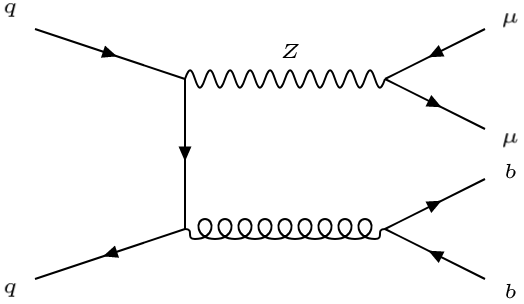
\includegraphics[scale=0.5]{Zbb_2.png}
				\caption{$q\overline{q}$ annihilation in conjunction with \newline the radiation of a gluon.}
				\label{Fig:SFigAnnihilationFeynman}
			\end{subfigure}
			\begin{subfigure}{.45\textwidth}
				\centering
				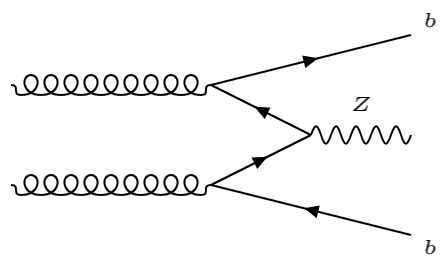
\includegraphics[scale=0.42]{Gluon_Pair.png}
				\caption{The final state produced by interactions \newline of a gluon pair.}
				\label{Fig:SFigGluonPairFeynman}
			\end{subfigure}
			\caption{A figure showing two possible mechanisms by which a Z$\rightarrow$($\mu\mu$)+bb final state can be achieved. }
			\label{Fig:FeynmanProcesses}
		\end{figure}
		
		\begin{comment}
		Another dominant process for this analysis is a single quark radiating both a Z boson and a gluon. Much like in the process of $q\overline{q}$ annihilation, the Z boson decays to two muons and the gluon produces a pair of b-quarks (with one being a standard b-quark, and the other its anti-particle). The Feynman diagram for this process can be seen in Figure \ref{Fig:SFigRadiationFeynman}. 
		\end{comment}
		
		
		Another dominant process for this production is a pair of gluons producing two quark-antiquark pairs. Each of the two gluons produces a bb pair, and interaction between the two pairs allows two of the quarks to annihilate and produce a Z boson (which later decays to two muons). The Feynman diagram for this process can be seen in Figure \ref{Fig:SFigGluonPairFeynman}. \par
		
		Finally, another process to be considered is that of the Compton process by which the interaction of a gluon with a single quark radiates a Z boson. It is this process that allows for the insight into the structure of the proton. At any one time, the content of a proton can be described by its PDF. \par
		
		The PDF of a given parton is a function of two variables: the fraction of the proton momentum carried by a parton ($x$), and the "scale" corresponding to the energy at which the parton is probed ($Q^{2}$). As the protons are collided inside the LHC beamline, the sea-quarks within the proton are able to interact with other partons such as valence quarks and gluons. For example in the case of Z$\rightarrow$($\mu\mu$)+b, the gluons and quarks interact via a hard process to produce a final state with one b-quark and a Z boson, which is subsequently detected by ATLAS. The cross section for this hard process can be written in the following form:
		
		\begin{comment}
		\begin{center}
			\begin{equation}
				\sigma (qg \rightarrow Zq) = \Sigma C_{i}^{P} (x,\alpha_{s}(Q^{2})) \otimes \tilde{f}_{i}(x,Q^{2},\alpha_{s}(Q^{2}))
			\end{equation}
		\end{center}
		With $C_{i}^{P}(x,\alpha_{s}(Q^{2}))$ as the perturbative calculable coefficient function, and $f_{i}(x,Q^{2},\alpha_{s}(Q^{2}))$ the probability to find a parton of type i carrying a fraction x of the proton momentum and $\tilde{f}_{i}(x,Q^{2},\alpha_{s}(Q^{2})) = xf_{i}(x,Q^{2},\alpha_{s}(Q^{2}))$ \cite{Article:PartonDistributions}. 
		\end{comment}
		
		\begin{center}
			\begin{equation}
			\frac{d\sigma}{dQ^{2}}=\sum_{i,j\in \{q,\overline{q},g\}}\int dx_{1}\int dx_{2}\; f_{i}(x_{1},Q^{2})f_{j}(x_{2},Q^{2})+f_{i}(x_{2},Q^{2})f_{j}(x_{2},Q^{2})\;\frac{d\hat{\sigma_{ij}}}{dQ^{2}}
			\end{equation}
		\end{center}
		
		With $\hat{\sigma}_{ij}$ as the cross section for (anti)-quarks and/or gluons, where $i$ and $j$ label the species of the colliding particle, and $f_{i}(x,Q^{2})$ the probability to find a particle of type $i$ carrying a fraction $x$ of the proton momentum\cite{Article:PartonDistributions}. When the process is detected, the momentum of the incident quarks can be calculated and used to perform a measurement of the proton PDF. PDFs are useful for calculating the cross sections of physical processes, and a measurement of Z$\rightarrow$($\mu\mu$)+b allows for a measurement of the proton PDF as well. The Feynman diagram for this process can be seen in Figure \ref{Fig:ZbbCompton}.
		
		\begin{figure}[h!]
			\centering
			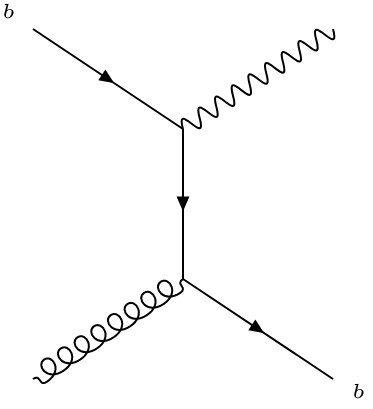
\includegraphics[scale=0.5]{Zbb_3.png}
			\caption{A figure showing the Feynman diagram for the Compton Process.}
			\label{Fig:ZbbCompton} 
		\end{figure}
			
		\subsection{Background Processes}
	
		As with the signal processes, the background process for Z$\rightarrow$($\ell\ell$)+b and Z$\rightarrow$($\ell\ell$)+bb are almost identical for both Z$\rightarrow$($ee$) and Z$\rightarrow$($\mu\mu$) with the only difference being the decay products of the Z boson. This section describes the processes for Z$\rightarrow$($\mu\mu$). \par
		
		The difficulty of Z$\rightarrow$($\mu\mu$)+bb analysis is in no small part due to the number of background processes that make a direct measurement difficult. In order to obtain a clear and accurate measurement of the signal process, there must be an equally clear understanding of the background processes such that any effect they have on a measurement of the signal process can be modelled and removed. \par
		
		The first and most common of these background processes is the top quark pair background. A pair of top quarks (specifically tt) are produced through one of many potential mechanisms, such as via a gluon interaction. Each top quark then undergoes a weak interaction to become a b quark, and produces a muon via a W boson and weak decay (as the overall charge of the process must be conserved). This results in the same final state as the Z$\rightarrow$($\mu\mu$)+bb signal process plus two additional neutrinos from the weak interaction of each top quark to a bottom quark. The Feynman diagram for this process can be seen in Figure \ref{Fig:SFigTtbarFeynman}. \par
		
		\begin{figure} [h!]
			\begin{subfigure}{.49\textwidth}
				\centering
				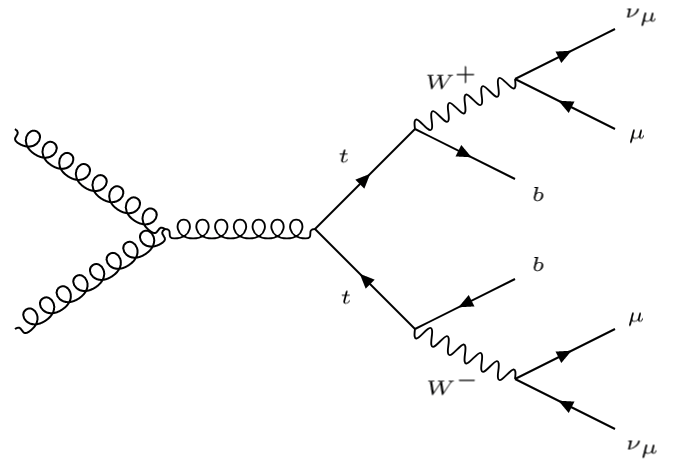
\includegraphics[scale=0.3]{Gluon_ttbar}
				\caption{The Top Quark Pair Production \newline background process.}
				\label{Fig:SFigTtbarFeynman}
			\end{subfigure}
			\begin{subfigure}{.49\textwidth}
				\centering
				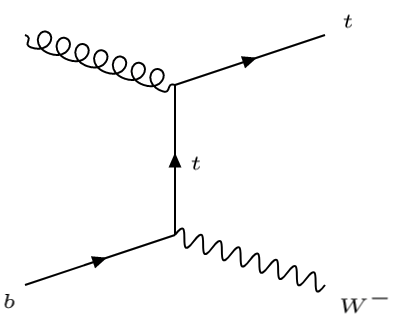
\includegraphics[scale=0.4]{Single_Quark}
				\caption{The Single Top background process.}
				\label{Fig:SFigWtFeynman}
			\end{subfigure}
			\caption{A figure showing the Feynman diagrams of Top Quark Pair Production and Single Top background production.}
			\label{Fig:FeynmanBackground1}
		\end{figure}
		
		\begin{comment}
		Similarly, instead of annihilating quarks exchanging a Z boson, a W boson can instead take its place. In this instance, instead of a top quark pair, a top quark and b-quark are produced. The top quark then decays to a second b-quark in the same manner as in the top quark pair background - the top quark changes flavour and the W boson decays to produce a muon and a neutrino. Unlike the top quark pair background, this single top background does not immediately appear to fulfil the final state of Z$\rightarrow$(\mu\mu)+bb. However, should this process occur in close proximity to another process in which a muon is produced, it could very easily be misidentified as a signal process. The Feynman diagram for this process can be seen in Figure \ref{Fig:SFigSTopFeynman}. 
		\end{comment}
		
		Another background process dependent on a charged current interaction is the single top background process. An incoming b-quark interacts with a gluon and experiences a weak interaction. A W boson is produced alongside a top quark, corresponding to the weak interaction of the b-quark. This results in the emission of only a single top quark, along with a W boson. This process can be seen in Figure \ref{Fig:SFigWtFeynman}. The final state is achieved by the weak interaction of first the top quark, which produces the necessary b-quark and an additional W boson, followed by the leptonic decay of two W bosons which produce a muon and a neutrino each. \par
		
		In addition to these background processes are the diboson background processes. In these interactions, annihilating quarks produce a combination of two bosons which produce	the required final state particles. The first of these processes is referred to as ZqqZll, in which both of the bosons produced are Z bosons. One Z boson decays to two leptons, and the second decays to two quarks. The most common source of this background in Z$\rightarrow$($\mu\mu$)+bb production is the case where one Z boson decays to two muons, and the other to two b-quarks. This	process can be seen in Figure \ref{Fig:SFigZqqZllFeynman}. \par
		
		The second of these diboson processes is referred to as WqqZll. This process is similar to the ZqqZll process, however in this instance only one of the produced bosons is a Z boson and the other is a W boson (as opposed to both being Z bosons). In this case, the W boson decays to two quarks, and	the Z boson to two leptons. The most common form that this background process takes in the Z$\rightarrow$($\mu\mu$)+bb analysis is the case where the W boson decays to a bottom quark and a charm quark, and the Z boson decays to produce two muons. This immediately fulfils the
		final state of the Z$\rightarrow$($\mu\mu$)+b processes, and can easily imitate the Z$\rightarrow$($\mu\mu$)+bb process if the charm quark is mistagged as a b-quark. These background processes (WqqZll and ZqqZll) are a small yet common background that is consistently present across the full energy range of the analysis. The Feynman diagram for these processes can be seen in Figure \ref{Fig:DibosonBackgroundFeynman}. \par
		
		
		\begin{figure}[h]
			\begin{subfigure}{.49\textwidth}
				\centering
				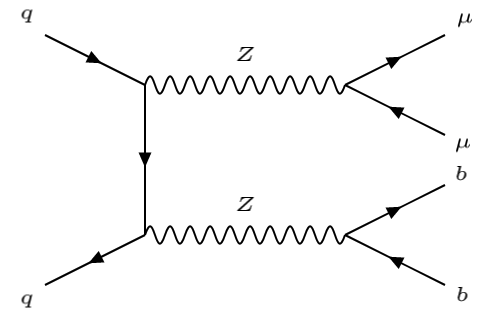
\includegraphics[scale=0.45]{ZqqZll}
				\caption{The ZqqZll background process.}
				\label{Fig:SFigZqqZllFeynman}
			\end{subfigure}
			\begin{subfigure}{.49\textwidth}
				\centering
				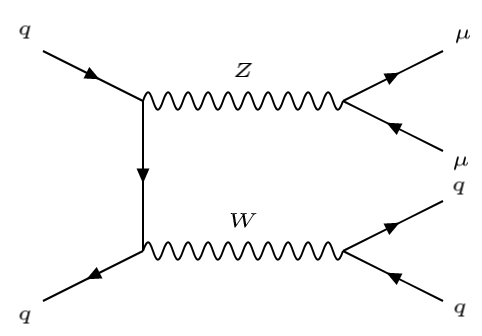
\includegraphics[scale=0.42]{WqqZll}
				\caption{The WqqZll background process.}
				\label{Fig:SFigWqqZllFeynman}
			\end{subfigure}
			\caption{A figure showing the Feynman diagrams for the WqqZll and ZqqZll background processes.}
			\label{Fig:DibosonBackgroundFeynman}
		\end{figure}  
		
		\begin{figure}[h!]
			\centering
			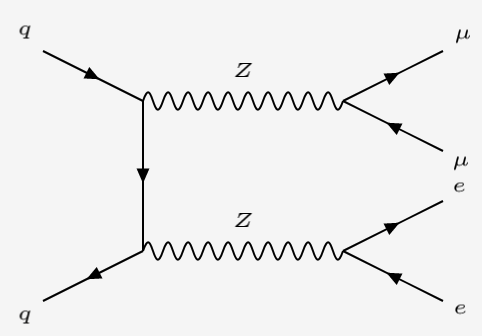
\includegraphics[scale=0.45]{ZZ4l}
			\caption{The ZZ4l background process.}
			\label{Fig:ZZ4lFeynman}
		\end{figure}
		
		
		In addition to the WqqZll and ZqqZll backgrounds mentioned above, there is an additional background process named ZZ4l which corresponds to an event where the two produced Z bosons decay into four leptons. The Feynman diagram for this process can be seen in Figure \ref{Fig:ZZ4lFeynman}. This background process occurs when one of the Z bosons produces two muons, and the other two electrons. Electrons produce jets along with
		electromagnetic showers within the electromagnetic calorimeters in ATLAS (see section 3.2.3), and a background process is found where this reconstructed jet is mistagged as a b-jet. \par
		
	\section{LHC and ATLAS}

		The source of all experimental data within this thesis is the ATLAS experiment at the Large Hadron Collider (LHC). The following chapters will provide an introduction to both the LHC and the ATLAS experiment with a primary focus on the subsystems of the ATLAS detector most relevant to this analysis. The data used in this thesis was collected during the second run of data collection by the LHC (appropriately named Run 2), which concluded in December of 2018. The third run of data collection will begin in 2021. 

		\subsection{LHC}

		100 meters beneath the site of the Conseil Européen pour la Recherche Nucléaire (CERN) at the French-Swiss border near Geneva, Switzerland lies the LHC. At approximately 27 kilometres in circumference, the LHC accelerates beams of protons to the highest energies in the world 
		reaching speeds greater than 99.9\% the speed of light \cite{LHCDesignV1, LHCDesignV2, LHCDesignV3}. 

		\subsubsection{Acceleration at the LHC}

		Beginning with it's initial flagship accelerator, CERN has constantly upgraded its accelerators and included the work of previous experiments in each new effort to collect even greater amounts of particle collision data. The full acceleration of the particle beams within the LHC is not reliant on a single static machine but a combined effort from multiple component accelerators, each of which further accelerates beams of particles to higher and higher energies prior to collision. Each particle accelerated by the LHC experiences not just a chain of particle accelerators, but a timeline of CERN's remarkable history.   
		
		This chain of accelerators begins with an ordinary container of hydrogen: atoms of hydrogen are extracted from the canister and subjected to an ionising electric field, stripping the hydrogen atoms of their electrons and leaving only the protons remaining. This ionised hydrogen gas is then immediately fed into the Linear Accelerator 2 (LINAC2), which accelerates the protons up to an energy of 50 MeV. LINAC2 has been in operation since 1978 after replacing the original Linear Accelerator 1 (LINAC1), and will itself be replaced by the Linear Accelerator 4 (LINAC4) in Run 3 to further upgrade the LHC \cite{LINAC4}. \par 
		
		Following their linear acceleration through LINAC2, the protons then enter the first of the four circular accelerators within the LHC acceleration chain: the Proton Synchrotron Booster (PSB). The PSB accelerates the protons to an energy of 1.4 GeV, before injecting them into the Proton Synchrotron (PS) which increases the energy of the protons to 25 GeV. The PS first accelerated protons on 24 November 1959, serving as CERN's first synchrotron. While the PS has been heavily modified from its original state, it still serves as a key piece of LHC operations over 60 years later. \par

		From the PS, the protons are then injected into the even more powerful Super Proton Synchrotron (SPS): far larger than the 688 m circumference of the PS, the SPS has a circumference of 7 km and almost 5 times as many electromagnets, capable of accelerating the protons to an energy of 450 GeV. The SPS originally operated as the principle collider of CERN's particle physics program when it came online in 1976 and was crucial in several key experiments in CERN's history, such as the Nobel-prize-winning discovery of the W and Z bosons in 1983 when the SPS ran as a proton-antiproton collider \cite{WBosonDiscovery, ZBosonDiscovery}. 

		The final step in the accelerator chain is the LHC itself, however the method of accelerating within the LHC differs slightly from the techniques of the previous circular accelerators. The protons from the SPS are injected to the LHC at two points instead of one in order to create two separate proton beams which circulate in opposite directions. These two distinct beams are each accelerated up to an energy of 6.5 TeV, allowing for a centre-of-mass energy of $\sqrt{s}$ = 13 TeV during Run 2. The full chain of LHC accelerators can be seen in Figure \ref{Fig:CERNRings}. \par

		\begin{figure}
			\centering
			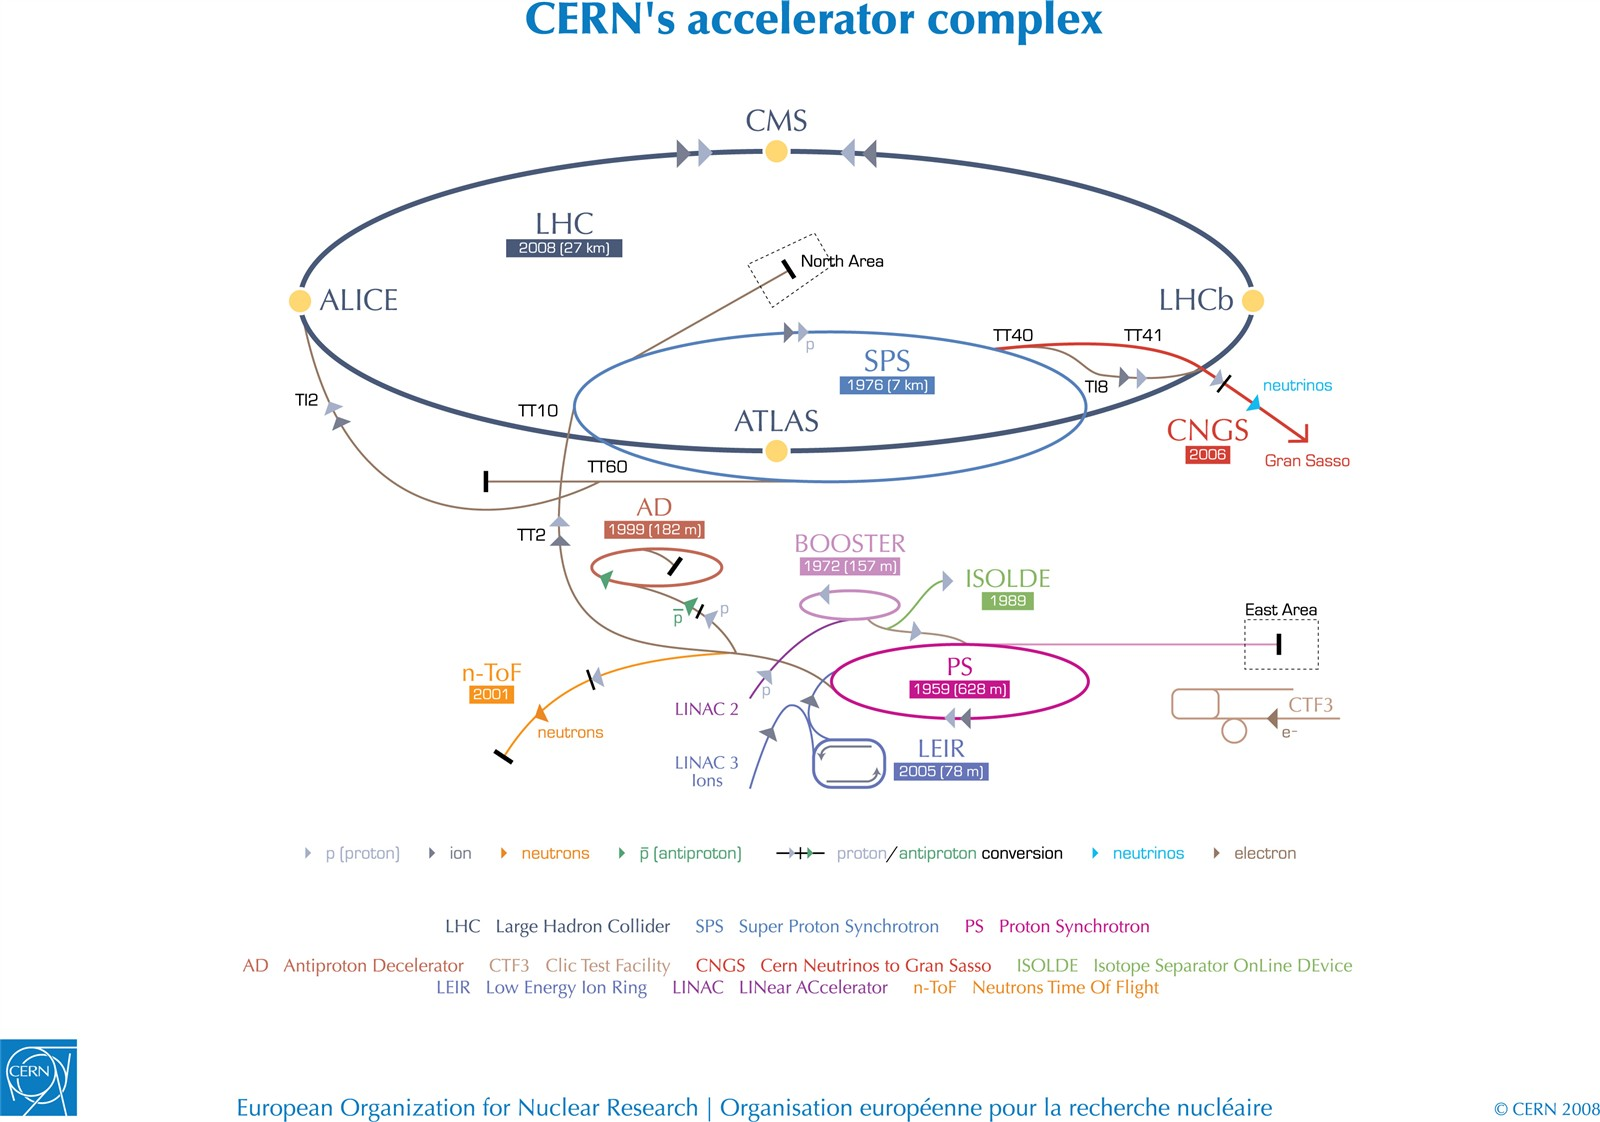
\includegraphics[scale=0.5]{LHC_Rings}
			\caption{A figure showing the arrangement and relative sizes of the accelerators within the LHC acceleration chain \cite{Article:CernComplex}.}
			\label{Fig:CERNRings}
		\end{figure}

		% End of rewrite to detector chapter 25/01/21

		Achieving the acceleration required to achieve these energies is no easy task. The tunnels in which the LHC resides were originally constructed for the Large Electron-Positron (LEP) collider \cite{LEPHistory, LEPDesign1, LEPDesign2, LEPDesign3}, a particle-antiparticle collider capable of accelerating two beams in opposite directions with the same magnetic field (due to the opposite charge between a charged particle and its respective antiparticle). The same method cannot be applied in the case of proton-proton collisions as the charge of each beam will be the same. Instead, the LHC uses its single magnet system to produced a pair of coupled magnetic fields which have an opposing polarity. \par

		The LHC does not, however, accelerate the particle beams at every point along its circumference. The LHC is composed of 8 octants, in which the LHC ring is actually a straight line. The curvature of the particle beams occurs at the boundaries of each octant, where 1232 powerful dipole magnets (each 15 metres long and with a weight of 35 tonnes) create a magnetic field of 8.3 T which bends the beams towards the centre of the LHC ring. These dipoles work in conjunction with 392 quadrupoles: magnets with alternating poles in a symmetrical layout that help focus the beam \cite{LHCMagnets}. In order to remain superconducting, these magnet are cooled with super-fluid Helium which allows the magnets to operate at 1.4 K. \par

		The straight sections of the LHC within each of the octants are referred to as "Points", and are numbered according to their position around the LHC ring. Each of these points can be seen in Figure \ref{Fig:CERNOctants}. Point 1, Point 2, Point 5, and Point 8 contain each of the interaction points (IPs) where the particle beams cross and interactions occur. Four large particle detectors of varying design are constructed at each of these IPs in order to observe the collisions that occur where the particle beams collide: two large general-purpose experiments (ATLAS \cite{ATLAS_Collab} and CMS \cite{CMSCollab}) at Point 1 and Point 5, the ALICE \cite{ALICECollab} experiment at Point 2 primarily examining heavy-ion collisions, and the LHCb \cite{LHCCollab} experiment at Point 8 primarily exploring flavour physics and CP-violation through bottom and charm quarks. \par

		\begin{figure}
			\centering
			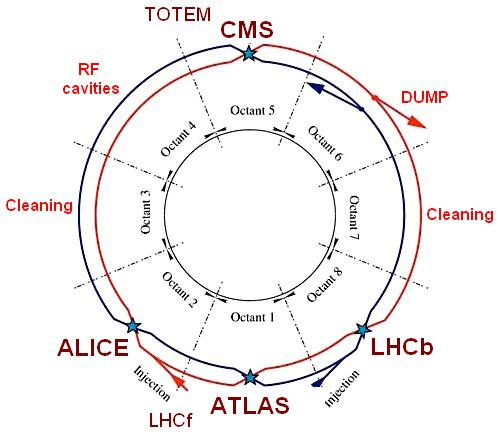
\includegraphics[scale=0.5]{LHC_Octants}
			\caption{A figure showing the arrangement of the LHC octants or "Points" \cite{Evans_2008}.}
			\label{Fig:CERNOctants}
		\end{figure}

		Point 3 and Point 7 contain the beam cleaning and collimation systems, essential systems that protect the components of the LHC. As proton beams travel around the LHC ring, they do not exist as a single some protons are unavoidably lost from the focussed central beam core and diffuse into a "beam halo", the fraction of the beam that will physically collide with the components of the LHC. These collisions from the beam halo can damage these components: for example, collisions with the LHC's superconducting magnets could cause a rise in temperature forcing the magnets out of a superconducting state (this is known as a magnet "quench") \cite{LHCCollimation1}. The collimator systems restrict the potential aperture of the beam, deliberately causing collisions with the beam halo to occur safely in the collimators (instead of in the LHC's more delicate subsystems) \cite{LHCCollimation2}. \par 

		The beam dump is located at Point 6, and is another important subsystem for the efficiency and safety of the LHC. When the particle beam within the LHC has served its purpose, the beam (or the remnants of it) needs to be safely removed from the LHC ring. The beam may also be dumped in the event of instability observed by the LHC or one of the detectors observing each of the IPs, or in the event of issues with one of the detectors. In the event that the beam needs to be dumped for any of these reasons, the LHC employs the use of kicker magnets that rapidly and safely diver the beam out of the LHC ring and into dump blocks: cylinders of graphite encased in concrete that can absorb the full energy of the beam without melting \cite{LHCDesignV2}. \par 
		
		The actual acceleration of the particle beam within the LHC occurs at the superconducting radio-frequency (RF) cavities located at Point 4. The LHC employs 8 RF cavities per beam, which use an alternating electric field to accelerate the beam through the cavity. By increasing the frequency of these oscillations, the particle beam can gradually increase to its maximum energy. Much like the dipole and quadrapole magnets used within the LHC, the RF cavities also operate at an extremely low temperature (4.5 K). The accelerating field provided by the RF cavities is 5 MV/m at 400MHz \cite{LHCRF}. Accelerating particles using the alternating electric field of the RF cavities causes the particle beam not to be a single continuous beam, but to instead be divided into \textit{bunches}.
		
		\subsubsection{Beam Structure}
		
		% 27/01/21

		When the particle beam passes through the RF cavities, some of the particles synchronize exactly with the RF frequency (these particles are aptly named "synchronous particles"). Particles that do not exactly synchronize with this frequency instead become clustered around the synchronous particle, and this travelling group of synchronized particles is referred to as a bunch. In order to allow for the necessary time for its subsystems to function correctly, the LHC beam is not a continuous stream of bunches but a combination of bunches and "missing" bunches (deliberate absences of bunches used primarily for timing). \par

		The nominal LHC beam consists of 2808 bunches, each consisting of $1.15 \times 10^{11}$ protons \cite{LHCDesignV1,LHCDesignV3}. The PS supplies particles to the SPS and LHC in the form of 72-bunch PS trains, with each bunch arriving 25ns apart \cite{LHCBeam}. When these bunches are accelerated by the SPS and enter into the LHC, they are arranged into the form of 3, 3, and then 4 PS trains. The very last PS train in the very last SPS batch is deliberately suppressed to allow time for the LHC extraction kicker magnets (required in the event of a beam dump) to rise. This bunch structure can be observed in Figure \ref{Fig:LHCBunches}. 

		\begin{figure}
			\centering
			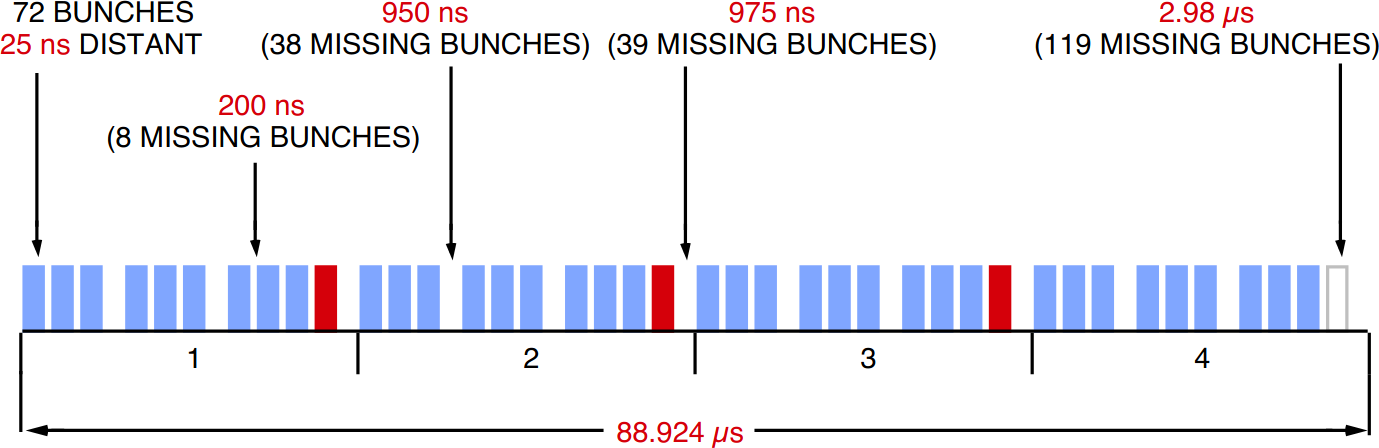
\includegraphics[scale=0.3]{LHC_Beam_Structure}
			\caption{A figure showing the arrangement of the PS trains within the final SPS batch injected into the LHC \cite{LHCBunches}.}
			\label{Fig:LHCBunches}
		\end{figure}

		% 28/01/21

		\subsubsection{Luminosity}

		In order to evaluate the performance of an accelerator, it is important to consider a metric that adequately describes the collisions taking place. In the case of accelerator physics \textit{luminosity}, a measure of how effectively an accelerator is able to deliver particle collisions, is used. For a process with a known cross section of $\sigma_{i}$, the event rate is given by:
		
		\begin{equation}
			\frac{\,dN}{\,dt} = \mathcal{L}_{i}\sigma_{i}
		\end{equation}

		where $\mathcal{L}_{i}$ is the instantaneous luminosity. The instantaneous luminosity (i.e. the luminosity of two colliding particle beams at any single instant) is useful for the measuring performance during stable collisions, although the quantity of integrated luminosity is typically more useful for measuring performance across a complete period of data collection. The integrated luminosity of an accelerator is defined as the integral of the accelerator's instantaneous luminosity with respect to time, i.e. the instantaneous luminosity at every instant or:
		
		\begin{equation}
			\mathcal{L}_{int} = \int \mathcal{L}_{i} \,dt 			
		\end{equation}

		Instantaneous luminosity is defined as: 

		\begin{equation}
			\mathcal{L}_{i} = \frac{N_{1}N_{2}kf\gamma}{4\pi\epsilon_{n}\beta^{*}}F
		\end{equation}
		
		where:

		\begin{itemize}
			\item $N_{1}$ and $N_{2}$ represent the number of protons within each colliding particle bunch
			\item $k$ is the number of bunches per beam
			\item $f$ is the frequency of the colliding beams (the nominal value of which is 11.245 kHz at the LHC)
			\item $\gamma$ is the relativistic Lorentz factor of the accelerated particles
			\item $\epsilon_{n}$ is the beam emittance (i.e. average spread of particles within the beam)
			\item $\beta^{*}$ is the beta function of the beam (i.e. the amount that the beam is "squeezed")
			\item $F$ is a geometric correction due to the crossing angle of the beams
		\end{itemize}

		Instantaneous luminosity is expressed in units of cm$^{-2}$s$^{-1}$. The peak instantaneous luminosity of the LHC was designed to reach a value of $1 \times 10^{34}$cm$^{-2}$s$^{-1}$, however this value has been exceeded and peak instantaneous luminosities of up to $2.1 \times 10^{34}$cm$^{-2}$s$^{-1}$ have been achieved. \par
		
		Integrated luminosity has units of cm$^{-2}$ but is more commonly expressed in units of inverse femtobarn fb$^{-1}$ where one barn (1 b) is equivalent to $1 \times 10^{-28} $m$^{-2}$. During Run 2 the ATLAS detector recorded a total of 139.9fb$^{-1}$ of luminosity usable for physics analyses corresponding to 3.2fb$^{-1}$ in 2015, 32.9fb$^{-1}$ in 2016, 43.7fb$^{-1}$ in 2017, and 60.1fb$^{-1}$ in 2018 \cite{ATLASLumiPublic}. \par
		
		This analysis uses the full 139.9fb$^{-1}$ luminosity of good data recorded by ATLAS during Run 2. The total amount of data recorded by ATLAS during Run 2 is greater than this figure at 146.9fb$^{-1}$, however not all of this data is suitable for physics analyses (such as in the event that not all detector subsystems are online). A visualisation of the luminosity delivered to and recorded by the ATLAS detector from the LHC can be seen in Figure \ref{Fig:ATLASLuminosity}.

		\begin{figure}
			\begin{subfigure}{.49\textwidth}
				\centering
				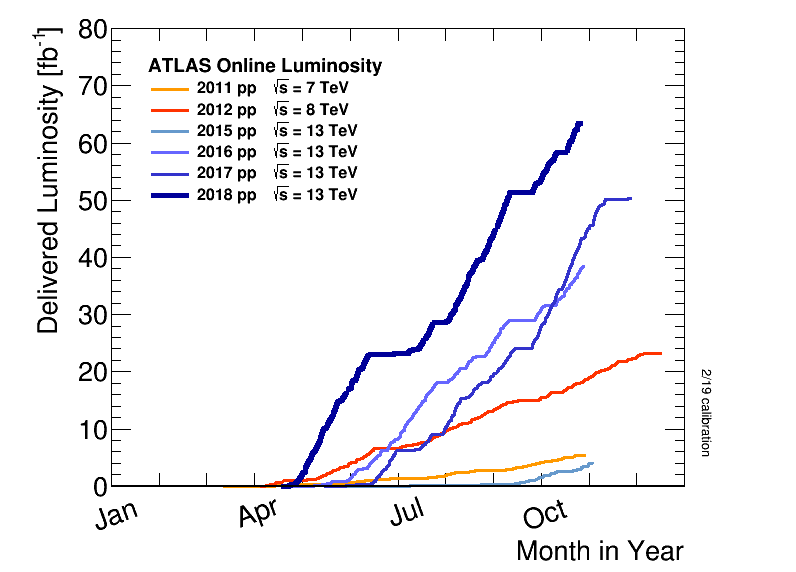
\includegraphics[scale=0.27]{ATLAS_Luminosity_Time.png}
				\caption{Delivered luminosity vs. time}
				\label{Fig:SFigATLASLuminosityTime}
			\end{subfigure}
			\begin{subfigure}{.49\textwidth}
				\centering
				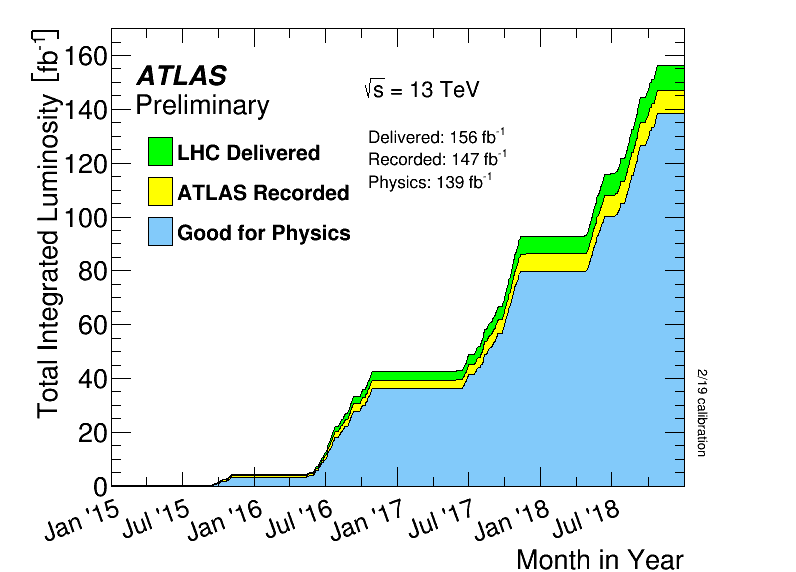
\includegraphics[scale=0.27]{ATLAS_Luminosity_Total.png}
				\caption{Total integrated luminosity vs. time}
				\label{Fig:SFigATLASLuminosityTotal}
			\end{subfigure}
			\caption{ (a) Cumulative luminosity versus month delivered to ATLAS during stable beams and for high energy p-p collisions. (b) Cumulative luminosity versus time delivered to ATLAS (green), recorded by ATLAS (yellow), and certified to be good quality data (blue) during stable beams for pp collisions at 13 TeV centre-of-mass energy in 2015-2018 \cite{ATLASLumiPublic}.}
			\label{Fig:ATLASLuminosity}
		\end{figure}

		%01/02/21

		\subsubsection{Pileup}\label{Section:Pileup}

		In the collision of two nominally filled bunches there are a total of $2.3 \times 10^{11}$ protons available to collide, allowing a high number of hard $pp$ interactions. Ideally the experiments at CERN would only record these hard interactions however this is not always the case, as additional interactions between bunches can occur. These additional interactions are referred to as pileup and can cause a multitude of issues in the reconstruction of hard events such as track mis-reconstructions, degradation of object resolution, and ambiguity in primary vertex location. \par
		
		Pileup can be categorised into two types:

		\begin{itemize}
			\item \textbf{In-time} pileup refers to other interactions within \textit{the same} bunch as the hard interaction.
			\item \textbf{Out-of-time} pileup refers to interactions within \textit{other} bunches relative to the hard interaction.   
		\end{itemize}

		Pileup is quantified by use of $\left\langle \mu \right\rangle$, the average number of interactions per bunch crossing. This value is corresponds to the mean of the poisson distribution of the number of interactions per crossing calculated for each bunch, calculated from the instantaneous per bunch luminosity which is given by the equation:

		\begin{equation}
			\mu = \frac{\mathcal{L}_{bunch}\times\sigma_{inel}}{f}
		\end{equation}

		where $\mathcal{L}_{bunch}$ is the per bunch instantaneous luminosity, $\sigma_{inel}$ is the inelastic cross section (taken to be 80 mb for $\sqrt{s}=13 TeV$ collisions), and $f$ is the LHC revolution frequency of 11.245 kHz. The full pileup profile of Run 2
		can be seen in Figure \ref{Fig:ATLASPileup}. The pileup profile uses the full 146.9fb$^{-1}$ of online data recorded by ATLAS during Run 2 as opposed to the 139.9fb$^{-1}$ of physics data, which can be seen in Figure \ref{Fig:SFigATLASLuminosityTotal}. 

		\begin{figure}
			\centering
			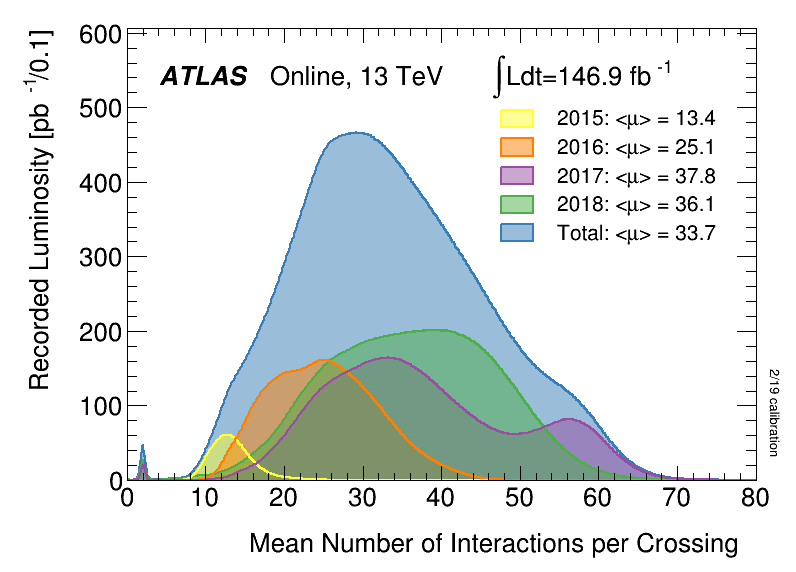
\includegraphics[scale=0.4]{ATLAS_Pileup_Run2.png}
			\caption{A figure showing the average interactions per bunch crossing for all ATLAS data recorded during Run 2 \cite{ATLASLumiPublic}.}
			\label{Fig:ATLASPileup}
		\end{figure}

		\subsection{ATLAS}

		The ATLAS (A Toroidal LHC ApparatuS) experiment \cite{ATLAS_Collab}, located at Point 1 of the LHC ring, is the largest general-purpose experiment at CERN. The design of ATLAS is carefully engineered in order to maximise its capabilities as a general-purpose particle detector \cite{ATLAS-TDR-01, ATLAS-TDR-02, Article:ATLASDesignPaper}. ATLAS is cylindrical in shape, with a length of 46 metres and a diameter of 25 metres. The immense scale of ATLAS can be difficult to picture without adequate reference: the diameter of ATLAS is 1 metre greater than the height of Buckingham palace, and its length is the same as the Statue of Liberty's height\footnote{The statue of liberty itself, excluding the 47 m pedestal that the statue stands upon.}. It would take a tower of 9 giraffes carefully lying head to hoof in the ATLAS cavern while wearing the appropriate personal protective equipment (PPE) to occupy the same length as the ATLAS detector\footnote{This would likely irritate the giraffes.}. 
		
		% The immense size of ATLAS can be difficult to picture without adequate reference:
		%\begin{itemize}
			%\item It would take a tower of nine giraffes, carefully balanced on each other's heads, to create a structure as tall as the length of the ATLAS detector\footnote{This would likely irritate the giraffes.}.
			%\item In would take over 56 billion tins of soup to completely fill the ATLAS detector's cavern, although it can be difficult to smuggle even a single tin past security\footnote{Allegedly.}.
		%\end{itemize}

		%02/02/21

		The ATLAS detector is constructed around the LHC beamline at Point 1 with its cylindrical geometry divided into two categories: the \textit{barrel} and the \textit{endcap}, which can be visualised as the sides and top/bottom of a standard cylinder respectively. The cylindrical design of the ATLAS detector allows almost full coverage of 4$\pi$ and forward-backward symmetry across the IP, hence the IP is located at the perfect centre of the barrel region in the heart of the detector. Particles originating from collisions at the IP travel outward and through different sub-systems, each sensitive to particular properties of various particles, in order to identify and reconstruct physics objects in each event. \par 

		%03/02/21

		The \hyperref[Section:InnerDetector]{Inner Detector (ID)}, the sub-system closest to the IP, tracks the path of all charged particles that pass through it. For particles travelling outward from the IP the next sub-system encountered are the calorimeter systems which aim to stop both hadronic and electromagnetic particles in order to measure their energy. Finally, the remaining particles from events at the IP pass through the outermost sub-system: the Muon Spectrometer (MS), which aims to identify and track the path of muons. All of these systems are subjected to a magnetic field generated by the ATLAS magnet systems: a solenoid magnet creates the field beyond the ID, and the eponymous toroidal magnet creates the magnetic field beyond the calorimeters. A cross section of ATLAS and these detector sub-systems can be seen in Figure \ref{Fig:ATLASDetector}.

		\begin{figure}
			\centering
			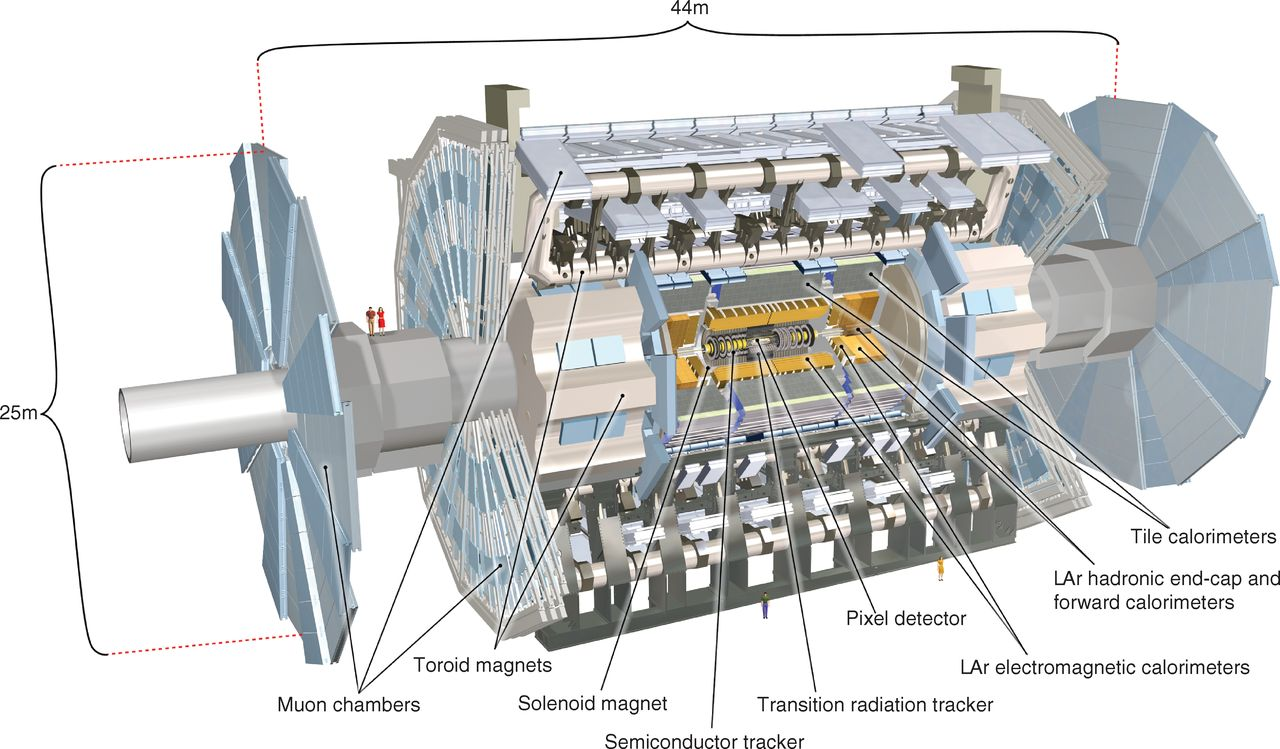
\includegraphics{ATLAS}
			\caption{A figure showing the subsystems of the ATLAS detector \cite{Article:ATLASDesignPaper}.}
			\label{Fig:ATLASDetector}
		\end{figure}

		\subsubsection{Coordinate System}

		In order to be able to accurately describe events relative to the detector and interaction point, ATLAS uses a well defined right-handed coordinate system. Taking the nominal IP as the origin, the $x$-axis points towards the centre of the LHC ring, the $y$-axis points vertically upwards, and the $z$-axis points along the direction of the beam pipe. A subtle yet crucial result of this coordinate system is the definition of the $x$-$y$ plane, which is tangential to the beam pipe (referred to as the \textit{transverse} plan). The nature of the fundamental colliding partons prevent the initial momentum in the $z$ direction from being known, however it is known that the partons have zero initial momentum in the transverse plane and therefore directional vector quantities such as momenta can be projected into the transverse plane. \par

		In addition, cylindrical coordinates are used to describe the geometry of the detector. The azimuthal angle, $\phi$, describes the angle around the beam direction in the transverse plane where $\phi = 0$ points in the same direction as the $x$-axis (i.e. towards the centre of the LHC ring). The polar angle, $\theta$, describes the angle from the beam direction in the $y$-$z$ plane where $\theta = 0$ points in the same direction as the $z$ axis (i.e. along the beam pipe). The final coordinate of the ATLAS coordinate system is the rapidity ($y$) or pseudorapidity ($\eta$). The rapidity of a particle is defined as: 

		\begin{equation}
			y = \frac{1}{2}\ln\left(\frac{E+p_{z}}{E-p_{z}}\right)
		\end{equation}

		where E is the particle's energy and $p_{Z}$ is the momentum of the particle in the $z$ axis. The pseudorapidity of a particle is defined in terms of the polar angle, $\theta$, as:

		\begin{equation}
			\eta = -\ln\tan\left(\frac{\theta}{2}\right)
		\end{equation}

		Pseudorapidity is typically used in place of $\theta$ as it is Lorentz invariant under a boost in the $z$-axis whereas $\theta$ is not. The rapidity and pseudorapidity are equivalent for massless particles and this holds true for particles with extremely small mass (several orders of magnitude lower than their average energy) such as electrons. The angular distance between two objects is described using the variable $\Delta R$, which is also Lorentz invariant under a boost in the $z$-axis. $\Delta R$ is defined by the relation:

		\begin{equation}
			\Delta R = \sqrt{ (\Delta\eta)^{2} + (\Delta\phi)^{2} }
		\end{equation}

		%04/02/21

		\subsubsection{The Magnet System}

		The ATLAS magnet system consists of four magnets: a single solenoid magnet \cite{ATLASSolenoidMagnet}, and three toroidal magnets \cite{ATLASBarrelToroid, ATLASEndcapToroid} (which contribute an important part of the ATLAS name). The central solenoid provides the magnetic field for the inner detector, and the toroidal magnets provide the magnetic field	for the muon system. The arrangement of the magnet systems within ATLAS can be seen in Figure . \par

		\begin{figure}
			\centering
			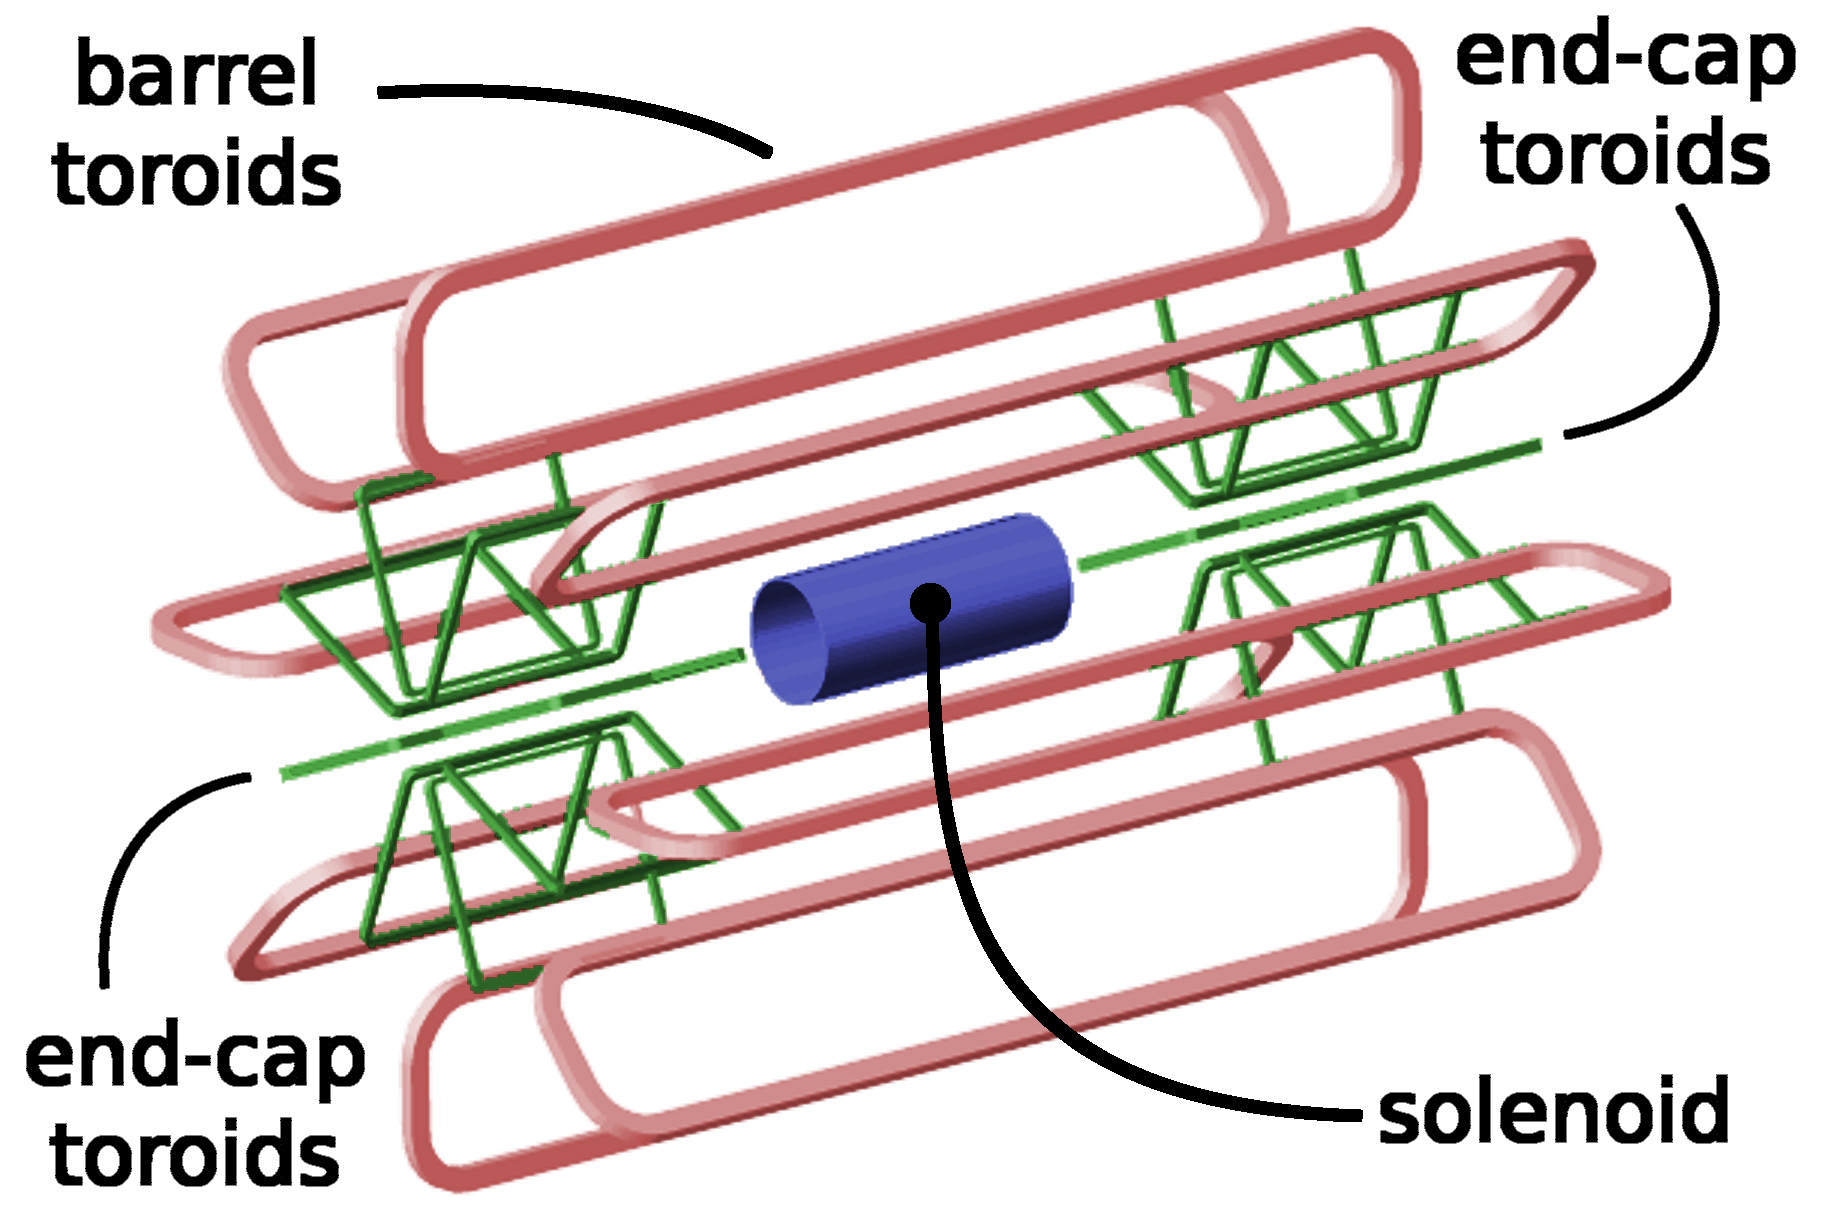
\includegraphics[scale=0.15]{Magnet_Layout.png}
			\caption{The relative location of the solenoid, barrel toroids, and endcap toroids \cite{ATLASToroids}. }
			\label{Fig:CernMagneticLayout}
		\end{figure}

		The solenoid magnet is named the Central Solenoid Magnet. It is aligned with the $z$-axis (i.e. the beam pipe) and exerts a 2T axial magnetic field which bends the path of charged particles within the inner detector. The magnet weighs 5 tonnes but is only 5 cm thick (which corresponds to 0.66 radiation lengths) in order to minimize the probability of particle interactions with the magnet itself. The solenoid is cooled to a temperature of 4.5 K in order to maintain its superconducting state, and is capable of storing a total of 38 MJ of energy. \par
		
		In the case of the toroidal magnets, there is one toroidal magnet located in the barrel region and one toroidal magnet in each endcap region. The magnetic fields produced by the toroids are orthogonal to each other, creating an overall magnetic field of 0.5 T in the barrel region and 1 T in each endcap. Together, these magnetic fields bend the path of muons in the outermost region of the detector. The position of each toroid's coils can be seen in Figure \ref{Fig:CernMagneticLayout}. Each magnet contains eight coils, however the coils for the barrel region are by far the largest with a length of 25.3 metres each whereas the length of the endcap coils are only 5 metres. Each endcap toroid weighs 240 tonnes and stores 0.25 GJ of energy, while the much larger barrel toroid weights a total of 830 tonnes and stores a total of 1.08 GJ of energy. 
		
		The shape of the magnetic field created within ATLAS by both the solenoid and toroidal magnet can be seen in Figure \ref{Fig:CernMagneticField}. 
		
		\begin{figure}
			\centering
			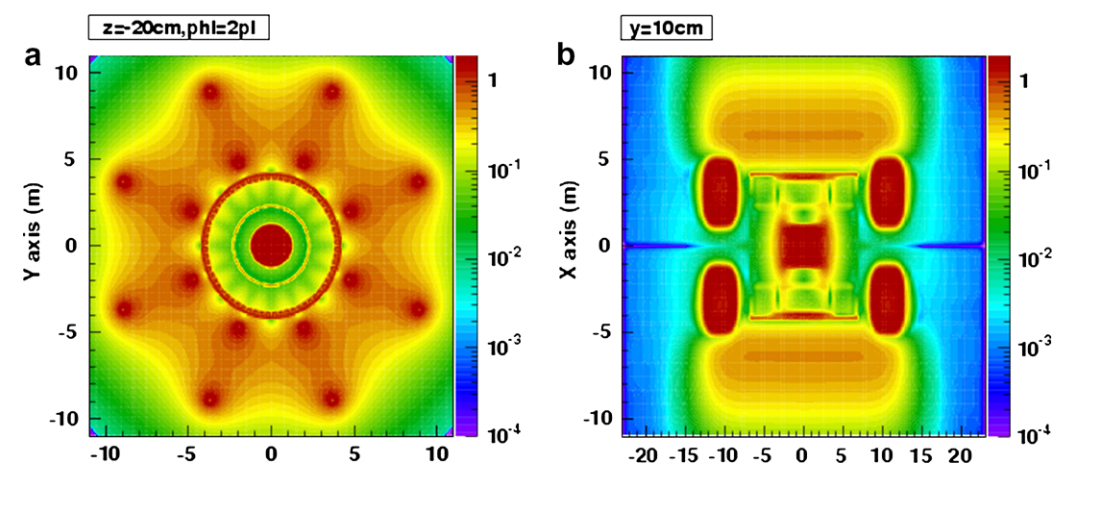
\includegraphics[scale=0.4]{Magnetic_Field}
			\caption{The shape of the magnetic field within the ATLAS detector. The left plot shows the magnetic field as if looking down the beamline. The right plot shows the magnetic field when viewed from above \cite{Article:CernMagnets}. }
			\label{Fig:CernMagneticField}
		\end{figure}

		% 05/02/21

		\subsubsection{Inner Detector}\label{Section:InnerDetector}

		The Inner Detector \cite{ATLASID1, ATLASID2} is the most central component of ATLAS providing precise measurements of both particle charge and momentum, in addition to tracking charged particles to a pseudorapidity range of $|\eta| < 2.5$. Using both an impact parameter, $d_{0}$, and a longitudinal impact parameter, $z_{0}$, the ID is able to characterise the primary vertex of each interaction. The parameter $d_{0}$ is defined as the distance between the vertex's point of closest approach and the $z$-axis, and the parameter $z_{0}$ is defined as the $z$-coordinate of the primary vertex's point of closest approach. A high precision measurement of the primary vertex is crucial to this analysis as the delayed secondary vertex of b-tagged events is an extremely important in their identification, and an excellent resolution for $d_{0}$ and $z_{0}$ allows for easier identification of b-hadrons and other particles with longer lifetime. 

		The ID consists of four subsystems which work in conjunction to track charged particles and perform high resolution measurements of their charge and momentum. These subsystems are the \hyperref[Section:IBL]{Insertable B-Layer (IBL)}, the \hyperref[Section:PixelDetector]{Pixel Detector}, the \hyperref[Section:SCT]{Semiconductor Tracker (SCT)}, and the \hyperref[Section:TRT]{Transition Radiation Tracker (TRT)}. The layout of these components within the ID barrel region can be seen in Figure \ref{Fig:InnerDetector}.  

		\begin{figure}
			\centering
			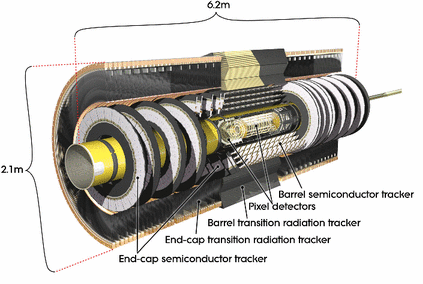
\includegraphics[scale=0.7]{Inner_Detector}
			\caption{A figure showing the layout of the ID within ATLAS \cite{Article:ATLASDesignPaper}. }
			\label{Fig:InnerDetector}
		\end{figure}

		The IBL, pixel detector, and SCT all operate through the use of pixel modules containing tens of thousands of silicon pixel sensors. As charged particles pass through the pixel sensors, they ionise with the silicon semiconductors, freeing electrons from atoms within the silicon and creating ion-electron pairs. By interpreting the resultant signal created at the points within these pixel modules that these ion-electron pairs are created, the path of the charged particles that pass through the ID can be measured. 

		\paragraph{The Insertable B-Layer (IBL)}\label{Section:IBL}

		The most central component of the ID is the IBL \cite{IBL-TDR} (positioned a mere R = 33.25 mm away from the beam pipe), which was added to ATLAS during the shutdown between Run 1 and Run 2. The IBL increases the resolution of $d_{0}$ and vertex measurements when compared with the pixel detector alone, which is an important addition due to the high pileup of Run 2 (which can easily obfuscate the primary vertex as discussed in Section \ref{Section:Pileup}). Each individual pixel is extremely small and has dimensions of $50 \mu m \times 250 \mu m$, which allows for a tracking resolution of 8 $\mu$m and 40 $\mu$m in the $x$-$y$ plane and $z$ direction respectively.  

		\paragraph{The Pixel Detector}\label{Section:PixelDetector}

		The pixel detector consists of three layers of concentric cylinders coaxial to the beam pipe, and three layers of endcap disks perpendicular to the beam pipe. The barrel layers are positioned at R = 50.5, 88.5, and 122.5 mm, with the endcap disks positioned at $z$ = 495, 580, and 650 mm. These components consist of a total of 1744 pixel modules \cite{ATLASPixel} with a thickness of 250 $\mu$m, each containing 47,232 pixels with dimensions of 50 $\mu$m $\times$ 400 $\mu$m. Each pixel module contains 16 front-end chips with 2880 readout channels equating to a total of 46,080 readout channels per module, however all 47,232 pixels are readout of each module (pixels in the inter-chip regions are ganged together to be readout). Overall, the pixel detector has over 80 million readout channels and provides a spatial resolution of 10 $\mu$m in the $x$-$y$ plane and a spatial resolution of 115 $\mu$m in the $z$-axis. 

		\paragraph{The Semiconductor Tracker (SCT)}\label{Section:SCT}

		\paragraph{The Transition Radiation Tracker (TRT)}\label{Section:TRT}

		% 08/02/21

		The inner detector is the most central component of ATLAS and aims to take extremely precise measurements of charged particles, with primary focus on momentum and vertex resolution. The inner detector covers a pseudorapidity range of $|\eta| <$ 2.5 and consists of the Pixel Detector, Semiconductor Tracker (SCT), and the Transition Radiation Tracker (TRT). These components can be seen in Figure \ref{Fig:InnerDetector}. \par
		
		Both the pixel detector and SCT consist of thousands of silicon sensors. The pixel detector consists of 1744 silicon wafers (each 250 $\upmu$m thick), and the SCT of 15912 silicon wafers (each 285±15 $\upmu$m thick). The charged particles that pass through the pixel detector and SCT ionise within the submodules’ silicon semiconductors, freeing electrons from atoms within the silicon and creating ion-electron pairs. By interpreting the resultant signal created at the points within these wafers that these ion-electron pairs are created, the path of the charged particles that pass through the inner detector can be measured 
		\cite{ATLAS-TDR-01, ATLAS-TDR-02, Article:ATLASDesignPaper}.
		\par
		
		
		\begin{comment}
		While these two systems can perform a preliminary identification of particles, and preliminary measurements of momentum, the most essential function of the pixel detector and SCT is its ability to identify and distinguish charged particle tracks. 
		\end{comment}
		
		
		 The inner detector performs several crucial functions within ATLAS: By performing measurements of charged particles that pass through the inner detector as their paths are bent by the magnet system, the inner detector can perform preliminary momentum measurements and track the paths of these charged particles throughout ATLAS. The measurements of momentum performed by the inner detector are supplemented by readings from other detector subsystems (such as energy deposits in the calorimeters), however the inner detector performs the most precise measurement of muon momentum. The paths measured by the inner detector provide excellent measurements of the tracks of charged particles, and are crucial for reconstructing events within ATLAS as they allow the detector triggers to correlate particle tracks to hits in other detector systems. By mapping hits in other detector subsystems with the paths tracked by the inner detector, it is possible to identify the kinematics and flavour of each particle travelling through ATLAS in order to fully describe each event. The inner detector is also responsible	for identifying the main interaction point of each collision, by tracing the particle tracks back to the point where they originate. \par
		
		The number of particle tracks that occur within each event is very high, and in order to perform these measurements the inner detector must have a very high spatial resolution. The pixel detector and SCT have spatial resolutions of 12$\upmu$m and 16$\upmu$m respectively, which is	essential to allow the detector to discern between the tracks of charged particles within the
		inner detector. The large number of events that occur within ATLAS every second can only be measured if the detector is able to accurately measure each involved particle, hence being	able to distinguish each event’s tracks and collision points is essential to all measurements
		performed by ATLAS. \par
		
		As charged particles pass through the TRT, they pass through drift tubes filled with a mixture of xenon, carbon dioxide, and oxygen gas. The charged particles emit transition radiation as they pass from the detector material into the gas, and also ionise the gas as they travel through it. The number of photons produced via transition radiation and
		electrons produced from EM-ionisation can be used to help distinguish between charged	particles such as electrons and pions. By observing which of the drift tubes detected a	signal, the TRT can supplement the measurement of the path of the charged particle	performed by the pixel detector and SCT. \par
		
		
		\begin{figure}
			\centering
			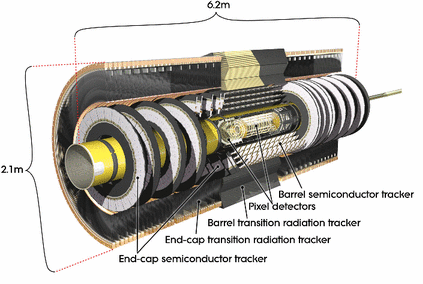
\includegraphics[scale=0.7]{Inner_Detector}
			\caption{A figure showing the layout of the inner detector within ATLAS \cite{Article:ATLASDesignPaper}. }
			\label{Fig:InnerDetector}
		\end{figure}

		\subsection{ATLAS}
		
		The ATLAS (A Toroidal LHC ApparatuS) experiment \cite{ATLAS-TDR-01, ATLAS-TDR-02, Article:ATLASDesignPaper} is one of the larger detectors in place along the circumference of the LHC beam pipe. ATLAS is a general purpose detector, and has been carefully engineered to maximise its potential in the probing of p-p collisions at the LHC. \par
		
		ATLAS and its components are described in a specific coordinate system using the interaction point and axis of the proton beam as a reference: The nominal interaction point (IP) is defined as the origin of the coordinate system, and the direction of the beam axis is defined as the positive z-axis. In addition to this, the positive y-axis is defined	as pointing vertically upwards in relation to the IP, and the positive x-axis as pointing	horizontally from the IP to the centre of the LHC ring. This automatically defines the x-y plane to be the plane tangential to the direction of the beam axis (z-axis). \par
		
		In this coordinate system, cylindrical coordinates are used to parametrise the geometry within the detector: the polar angle $\theta$  is the angle from the beam axis and the azimuthal angle $\phi$ is the angle around the beam direction in the x-y plane. The pseudorapidity is then defined in terms of $\theta$ as $\eta = - \ln[\tan(\theta/2)]$. Using this, the distance between two points in $\eta-\phi$ space can be defined as $\Delta R =	\sqrt{\Delta\eta^{2}+\Delta\phi^{2}}$. \par
		
		In order to maximise the acceptance in pseudorapidity and cover the largest azimuthal angle possible (i.e. to maximise detection coverage of any events that occur within the detector), ATLAS is symmetrical with respect to the path of the accelerated protons. The	ATLAS detector operates using a combination of several subsystems, each of which can
		be seen in Figure \ref{Fig:ATLASDetector}. \par
		
		\begin{figure}
			\centering
			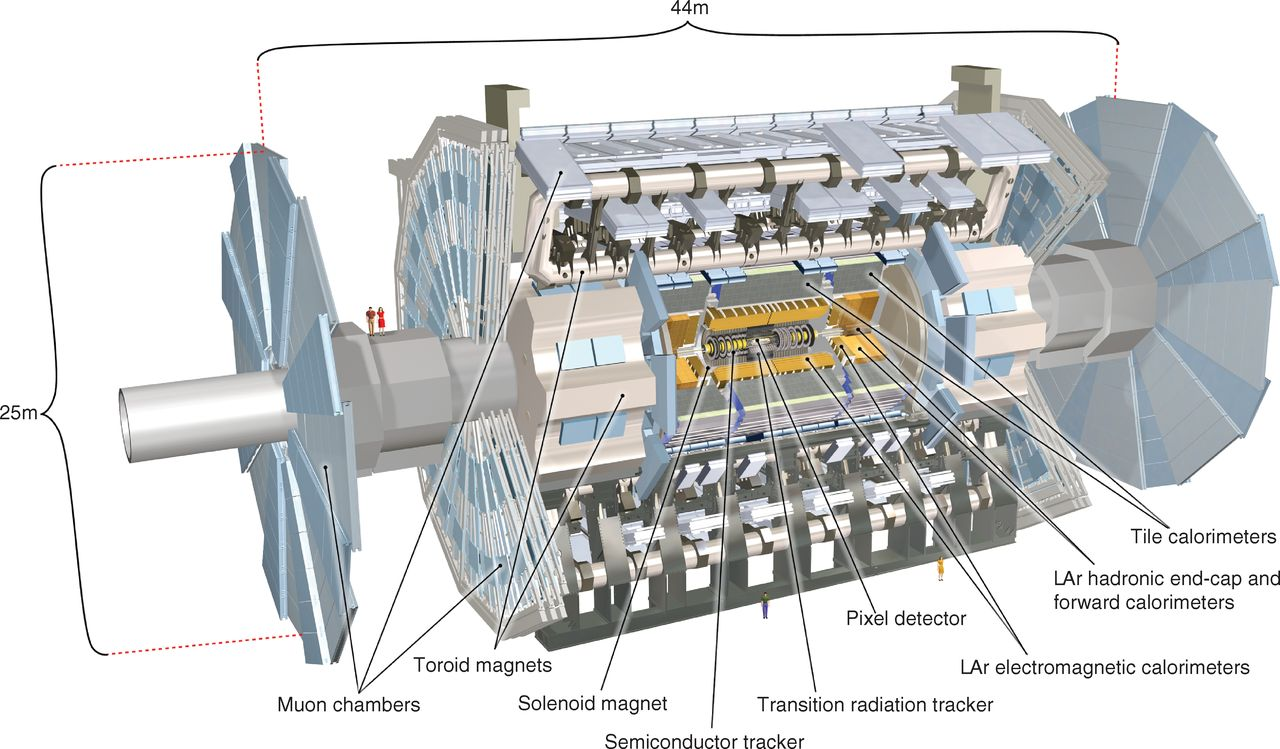
\includegraphics{ATLAS}
			\caption{A figure showing the subsystems of the ATLAS detector \cite{Article:ATLASDesignPaper}.}
			\label{Fig:ATLASDetector}
		\end{figure}
		
		These subsystems are layered outwards from the central interaction points, largely in the form of concentric cylinders (however this is not true for every component which will be discussed in the following sections). These systems can be	organised into four categories based on their function: the magnet system, the inner detector, the calorimeter system, and the muon system. Together with the trigger system, these components are designed to allow ATLAS to operate with the highest possible efficiency. \par
		
		\subsubsection{Magnet System}
		
		The ATLAS magnet system consists of four magnets: a single solenoid magnet, and three toroidal magnets (which contribute an important part of the ATLAS name). The central solenoid provides the magnetic field for the inner detector, and the toroidal magnets provide the magnetic field	for the muon system. \par

		The solenoid magnet is named the Central Solenoid Magnet and serves the purpose of bending the path of charged particles within the inner detector so that their momentum	may be measured. The most important function of this system for this analysis is the 2T	axial magnetic field that it exerts within ATLAS. The magnet weighs 5 tonnes, and is aligned with the z-axis of the beam pipe. The solenoid magnet is also capable of storing	a total of 38MJ of energy. \par
		
		The toroidal magnets have different designs for their varying purposes. The first is the end-cap magnets: large, doughnut shaped magnets that rest at either end of the detector and provide the magnetic field in the end-cap regions of the muon system. The second is the barrel toroid - longer, 25.3m toroidal coils that span the length of the muon system
		and provide a constant toroidal magnetic field to that system. The contributions of the barrel and end-cap toroids to the toroidal field around the muon detectors is as follows: 0.5T from the barrel toroid, and 1T from each of the end-cap toroids. Each end-cap magnet weighs 240 tonnes and stores 0.25GJ of energy. The barrel toroid consists of eight
		individual coils stored within vacuum vessels that surround both the end-cap magnets and the calorimeter systems. The barrel toroid weighs a total of 830 tonnes, and stores a total of 1.08GJ of energy. The shape of the ATLAS magnetic field can be seen in Figure \ref{Fig:CernMagneticField}. 
		\cite{ATLAS-TDR-01, ATLAS-TDR-02, Article:ATLASDesignPaper}
		
		\begin{figure}
			\centering
			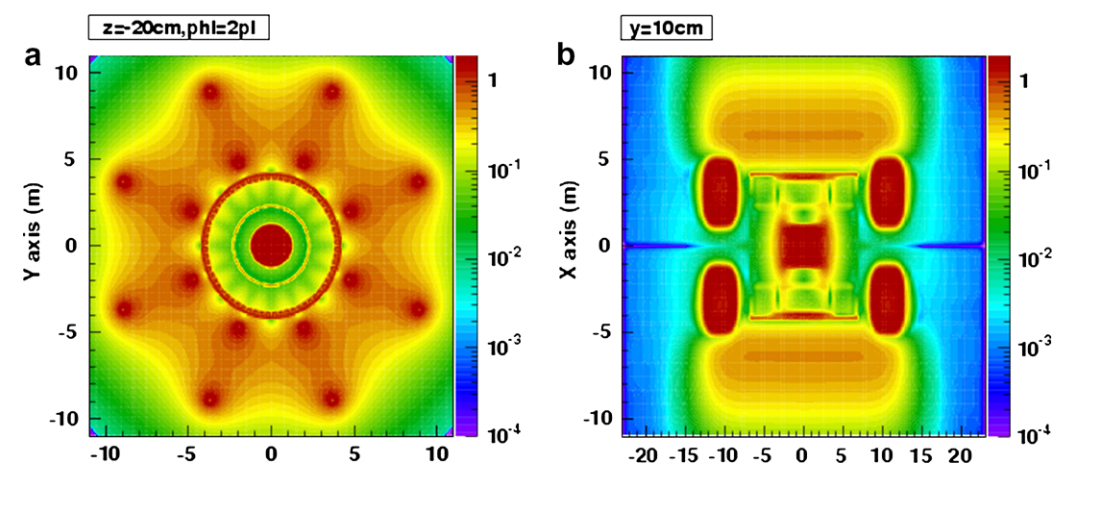
\includegraphics[scale=0.4]{Magnetic_Field}
			\caption{The shape of the magnetic field within the ATLAS detector \cite{Article:CernMagnets}. }
			\label{Fig:CernMagneticField}
		\end{figure}
		
		\subsubsection{Inner Detector}
		
		The inner detector is the most central component of ATLAS and makes the most immediate measurements after a collision such as those of the primary and secondary vertex, and of particle momentum. The inner detector covers a pseudorapidity range of $|\eta| <$ 2.5	and consists of the Pixel Detector, Semiconductor Tracker (SCT), and the Transition
		Radiation Tracker (TRT). These components can be seen in Figure \ref{Fig:InnerDetector}. \par
		
		Both the pixel detector and SCT consist of thousands of silicon sensors. The pixel detector consists of 1744 silicon wafers (each 250 $\upmu$m thick), and the SCT of 15912 silicon wafers (each 285±15 $\upmu$m thick). The charged particles that pass through the pixel detector and SCT ionise within the submodules’ silicon semiconductors, freeing electrons from atoms within the silicon and creating ion-electron pairs. By interpreting the resultant signal created at the points within these wafers that these ion-electron pairs are created, the path of the charged particles that pass through the inner detector can be measured 
		\cite{ATLAS-TDR-01, ATLAS-TDR-02, Article:ATLASDesignPaper}.
		\par
		
		
		\begin{comment}
		While these two systems can perform a preliminary identification of particles, and preliminary measurements of momentum, the most essential function of the pixel detector and SCT is its ability to identify and distinguish charged particle tracks. 
		\end{comment}
		
		
		 The inner detector performs several crucial functions within ATLAS: By performing measurements of charged particles that pass through the inner detector as their paths are bent by the magnet system, the inner detector can perform preliminary momentum measurements and track the paths of these charged particles throughout ATLAS. The measurements of momentum performed by the inner detector are supplemented by readings from other detector subsystems (such as energy deposits in the calorimeters), however the inner detector performs the most precise measurement of muon momentum. The paths measured by the inner detector provide excellent measurements of the tracks of charged particles, and are crucial for reconstructing events within ATLAS as they allow the detector triggers to correlate particle tracks to hits in other detector systems. By mapping hits in other detector subsystems with the paths tracked by the inner detector, it is possible to identify the kinematics and flavour of each particle travelling through ATLAS in order to fully describe each event. The inner detector is also responsible	for identifying the main interaction point of each collision, by tracing the particle tracks back to the point where they originate. \par
		
		The number of particle tracks that occur within each event is very high, and in order to perform these measurements the inner detector must have a very high spatial resolution. The pixel detector and SCT have spatial resolutions of 12$\upmu$m and 16$\upmu$m respectively, which is	essential to allow the detector to discern between the tracks of charged particles within the
		inner detector. The large number of events that occur within ATLAS every second can only be measured if the detector is able to accurately measure each involved particle, hence being	able to distinguish each event’s tracks and collision points is essential to all measurements
		performed by ATLAS. \par
		
		As charged particles pass through the TRT, they pass through drift tubes filled with a mixture of xenon, carbon dioxide, and oxygen gas. The charged particles emit transition radiation as they pass from the detector material into the gas, and also ionise the gas as they travel through it. The number of photons produced via transition radiation and
		electrons produced from EM-ionisation can be used to help distinguish between charged	particles such as electrons and pions. By observing which of the drift tubes detected a	signal, the TRT can supplement the measurement of the path of the charged particle	performed by the pixel detector and SCT. \par
		
		
		\begin{figure}
			\centering
			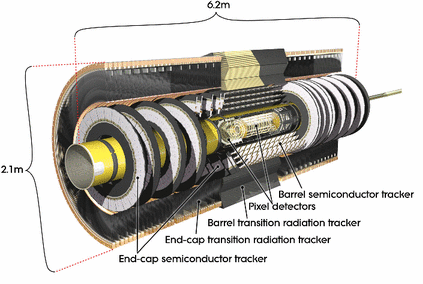
\includegraphics[scale=0.7]{Inner_Detector}
			\caption{A figure showing the layout of the inner detector within ATLAS \cite{Article:ATLASDesignPaper}. }
			\label{Fig:InnerDetector}
		\end{figure}
		
		\subsubsection{Calorimeter System}
		
		Two different calorimeters surround the inner detector and solenoid magnet to continue the measurements of particles travelling through ATLAS: the Electromagnetic Calorimeter and Hadronic Calorimeter (each of which consists of multiple pieces). The ATLAS calorimeters are sampling calorimeters, meaning that they work via a combination of absorber (or sampling) materials which cause an interaction within the module, and an
		active material which produces a signal which is interpreted by ATLAS. The electromagnetic	calorimeter consists of lead absorbers with a liquid argon (LAr) activate material, and the hadronic calorimeter consists of steel absorbers with scintillators as the active material. The layout of the calorimeter system can be seen in Figure \ref{Fig:ATLASCalorimeters}. \par
		
		By working in tandem, the two calorimeters perform measurements of the energy deposited by the travelling particles, regardless of whether the particles are charged or neutral. Naturally, the electromagnetic calorimeter focuses on absorbing the energy produced in electromagnetic showers, and the Hadronic calorimeter absorbs energy from hadronic
		showers. Both calorimeters surround the beam pipe, fully covering the azimuthal angle	$\phi$. Each calorimeter system is a combined effort from several pieces in order to cover a large range of $|\eta| <$ 4.9. \par
		
		In order to allow ATLAS to operate at maximum efficiency, incoming particles that cause electromagnetic and hadronic showers need to be fully contained within the calorimeters. This ensures that ATLAS can study the full shower, and prevents particles other than muons from penetrating through to the muon system. This is achieved by constructing the	calorimeters to be an appropriate depth: the EM calorimeter is designed to be between	24 and 27 radiation lengths (X$_{0}$) deep, and the hadronic calorimeter is designed to be 10 nuclear interaction lengths ($\uplambda$) thick. X$_{0}$ and $\uplambda$ represent the differing manners in which EM and hadronic particles lose energy, and for each unit one radiation/interaction length
		is the distance at which a travelling particle decreases to 1/e of its original energy.\par
		
		The electromagnetic calorimeter consists of three parts: a barrel calorimeter and two end-cap calorimeters, with the barrel calorimeter covering 0 $< |\eta| <$ 1.475 and the end-cap calorimeters covering 1.375 $< |\eta| <$ 3.2. All of these calorimeters follow the geometry of
		an accordion, allowing full coverage of $\phi$ within the EM calorimeter without any spaces 
		\cite{ATLAS-TDR-01, ATLAS-TDR-02, Article:ATLASDesignPaper}. \par 
		
		EM particles passing through the EM calorimeter interact with lead absorbers, creating a shower of lower energy particles. The incoming particles produce photons via the bremsstrahlung process (or other means such as a pion producing two photons), which then produce additional electrons via pair production. This alternating process of emitting
		photons which then produce electrons continues until the total energy of the shower is below that required for pair production to occur. Muons are capable of radiating photons as they pass through the EM calorimeter, which may produce additional secondary objects themselves. Typically these jets will be far less energetic than those produced by incoming electrons and photons,
		as photons radiated by muons carry only a small portion of the incident muon’s energy. \par
		
		The EM calorimeter is fine-granulated, so that the calorimeter can reconstruct each showering particle. EM showers can easily have many simultaneous interactions (such as a pion decaying into two photons within proximity of an additional photon), and it is important
		to be able to distinguish between these occurrences for a detailed analysis. \par
		
		Once these incident particles have lost enough energy to be beneath the energy requirement to produce an EM shower, energy loss mainly occurs by ionisation of the LAr within the EM calorimeter which frees additional electrons. The electrons produced within the LAr are attracted toward a copper electrode where they are interpreted into an electronic signal which reveals the amount of energy
		deposited by the original incident EM particle. Within the EM calorimeter, the thickness	is $>$ 22 X$_{0}$ thick in the barrel calorimeters and $>$ 24 X$_{0}$ in the end-cap calorimeters. \par
		
		\begin{figure}
			\centering
			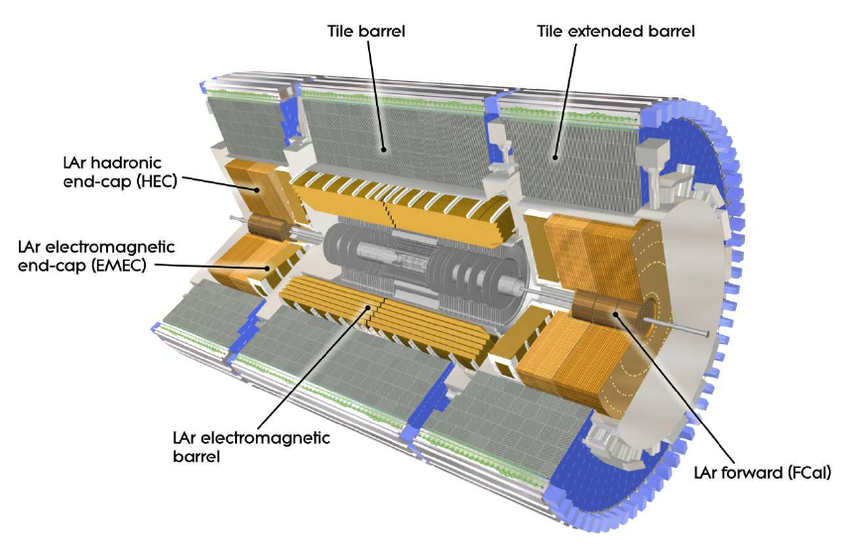
\includegraphics[scale=0.4]{ATLAS_Calorimeters}
			\caption{A figure displaying the arrangement of the electromagnetic and hadronic calorimeters within the ATLAS detector \cite{Article:ATLASDesignPaper}.}
			\label{Fig:ATLASCalorimeters} 
		\end{figure} 
		
		The hadronic calorimeter is similarly consisting of three distinct parts: the hadronic tile calorimeter, LAr forward calorimeter (FCal), and the LAr hadronic end-caps (HEC). One large central barrel cylinder and two smaller extended barrel cylinders make up the tile calorimeter - a system of alternating steel absorbers and scintillating
		plates. \par
		
		Travelling hadrons interact with the nuclei of the steel absorbers, producing additional particles. These particles then continue to interact, producing large showers of interactions. As these showers continue into the hadronic calorimeter, charged particles produce
		photons within the scintillating material. The photons emitted are carried to photomultiplier tubes via wavelength shifting fibres, where the photomultiplier tubes (PMTs) convert the photons into an electronic signal. By measuring the intensity of the light that creates the electronic signal, the energy deposited by the travelling hadron can be
		measured. The barrel tile calorimeter has a total thickness of 9.7 $\uplambda$ for the combination of both the central barrel cylinder and extended barrel cylinders 
		\cite{ATLAS-TDR-01, ATLAS-TDR-02, Article:ATLASDesignPaper}. \par 
		
		In order to be able to accurately measure the energy of incoming particles, the barrel calorimeter is required to have a high energy resolution ($\sigma/E$). In an event where energy is deposited within a calorimeter, a calorimeter with high energy efficiency is better equipped to reconstruct the energy of the original event (and therefore high energy resolution was an important factor considered during the design of ATLAS). Using electron test beam measurements, the energy resolution of the EM barrel calorimeter was found to be $\sigma/E = 10\%/\sqrt{E} \oplus 2\%$ (where the simple $\oplus$ represents a quadratic sum) \cite{Article:ECALCalibration}. 
		
		In addition to the barrel tile calorimeter which covers a range of 0 $< |\eta| <$ 1.0 are the HEC and the FCal, which maximise the $\eta$ coverage of the calorimeters. The FCal is positioned in the very far forward and backward regions of 3.1 $< |\eta| <$ 4.9. The FCal consists of three modules, each containing a layer of a metal absorber and electrodes, plus LAr as the active detecting material. The first module is made of copper in order to allow electromagnetic measurements, and the other two layers are made of tungsten to allow measurements of hadronic interactions in the same method as the tile calorimeter. The total depth of the FCal is 10 interaction lengths. \par
		
		The HEC overlaps with the tile calorimeter and the FCal in order to ensure full  coverage. The HEC uses copper as its absorber and LAr as its active material, covering a range of 1.5 $< |\eta| <$ 3.2. Together these three pieces form the hadronic calorimeter and cover the
		pseudorapidity range of 0 $< |\eta| <$ 4.9. In test beam studies, the energy resolution of hadrons in the tile calorimeter was measured to be $\sigma/E=52.9\%/\sqrt{E} \oplus 5.7\%$ \cite{Article:FCALCalibration}. 
		
		\subsubsection{Muon System}
		
		The final ATLAS detector subsystem is the muon system which rests outside the calorimeter system and inner detector. The muon system’s role is to measure the path and momentum of muons in the pseudorapidity range of $|\eta| < $ 2.7. The measurements in this region are dependent upon the toroidal magnets, which allow the tracks of charged particles able to penetrate the other detector systems to be measured. The barrel toroid provides the magnetic field in the region $|\eta| <$ 1.4, the end-cap toroids provide the field in the region 1.6 $< |\eta| <$ 2.7, and the two work in tandem to produce the field in the transition region of 1.4 $< |\eta| <$ 1.6. \par
		
		The bending of the muon tracks allows for measurements to be made in a similar fashion	as to within the inner detector, and this is coupled with additional measurements from four components: precision measurements from monitored drift tubes (MDT) and cathode strip chambers (CSC), and trigger measurements from resistive plate chambers (RPC) and thin gap chambers (TGC).\par
		
		
		\begin{figure}
			\centering
			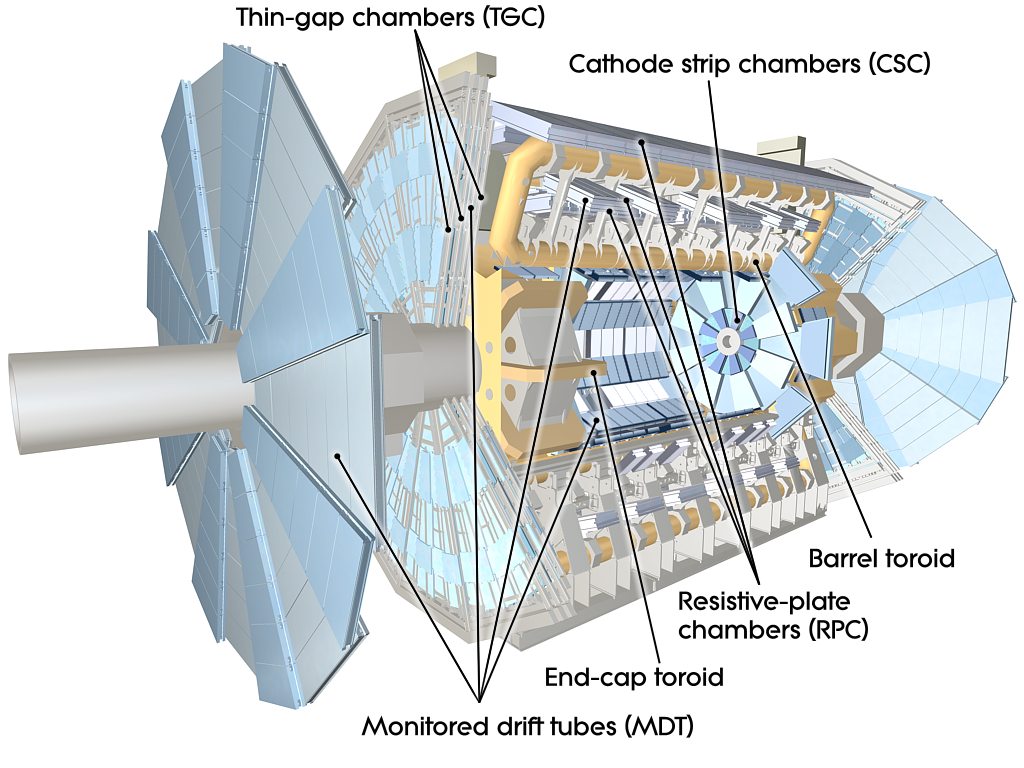
\includegraphics[scale=0.3]{Muon_System}
			\caption{A figure showing the position of the individual muon systems within ATLAS \cite{Article:ATLASDesignPaper}.}
			\label{Fig:MuonSystem}
		\end{figure}
		
		The CSCs are located in the forward regions of 2 $< |\eta| <$ 2.7, as they are capable of dealing with the highest particle fluxes of up to 1000 Hzcm$^{-2}$. The MDTs are located cover the region $|\eta| <$ 2.7 and consist of layers of drift tubes: cylinders containing a mixture of argon and carbon dioxide gas, with a wire at the centre. Muons that travel through the drift tubes ionise the gas and produce electrons and ions which drift to the wire and edge of the drift tube respectively, and are interpreted as an electronic signal.By observing the amount of ionisation, particle drift time, and the time and position of each emitted signal, the momentum of the travelling muon can be measured. The layout of the muon system can be seen in Figure \ref{Fig:MuonSystem}. \par
		
		The RPCs and TGCs serve as fast trigger chambers, able to provide track information approximately 10ns after a particle penetrates. The RPCs are located in the barrel covering the range $|\eta| <$ 1.05, and the TGCs in the end-cap covering the region 1.05 $< |\eta| <$ 2.4. While the CSCs and MDTs record precision measurements regarding the incident muons, the RPCs and TGCs are utilised for providing information to the trigger systems. \par
		
		The RPCs are gaseous parallel electrode-plate detectors consisting of two resistive plates separated by a 2mm gas gap: incoming muons are deflected towards the anode of the RPC allowing for a signal readout. TPCs are multi-wire proportional chambers arranged into layers positioned around the MDTs and in front of the most inward positioned tracking layer. As incident muons penetrate the sub layers within the TPCs, a signal is emitted if a muon is detected in multiple layers of the detector. The time and position of where this signal originates corresponds to a muon hit, and aids the trigger system in identifying muon events 
		\cite{ATLAS-TDR-01, ATLAS-TDR-02, Article:ATLASDesignPaper}. \par 
		
		
		\subsubsection{Trigger System}
		
		The trigger system’s function is to manage the enormous number of collisions that occur within ATLAS every second, identifying events that correspond to the expected standards of ATLAS, and ignoring those that do not. This operation is performed by a combination of a hardware based Level 1 (L1) trigger and a software based High Level Trigger (HLT). \par
		
		The L1 trigger uses information from the calorimeters and muon system to identify regions of interest within the recorded data, and performs the first classification of the data recorded, before passing events are sent to the HLT. This operation takes place within 2.5$\mu$s, and reduces the event rate from 40MHz to less than 75kHz (although it is
		still possible to operate with up to 100kHz output rate from the L1 trigger). \par
		The HLT runs on a dedicated server farm, and uses high speed algorithms to further refine events in the region of interest that pass the L1 trigger. The HLT reduces the event rate further to 1kHz, processing each event in an average of 0.2s. \par
		
		\bibliographystyle{Thesis.bst}
		
		\bibliography{Prog_2}
		
		\newpage
		\pagenumbering{gobble}
		
		\large \bf \underline{Thesis plan}
		
		\bigskip
		
		\small \bf \underline{November 2019 - January 2020: Framework Development and Validation}
		
		\normalfont The multiple frameworks in the Z+hf analysis group currently show promise, but are not yet ready for full analysis. During this time period, it would be ideal to achieve the following goals: 
		
		\begin{itemize}
		\item Implement systematic uncertainties. Currently the ZHFReader code has functionality for the systematics, but they do not function correctly
		\item Validate between the frameworks. This requires participation within the analysis groups and it not fully attainable by working alone, however there are some steps that could already be taken to build on the progress made during the "coding days @ CERN" event
`		\end{itemize}

		\bf \underline{February 2020 - April 2020: \newline Production of top and multijet enriched control regions}
		
		\normalfont Measurement of prevalent backgrounds can be performed in order to reduce uncertainties before unfolding, or even to avoid propagating negligible backgrounds through the entire analysis. During this time period, it would be ideal to achieve the following goals: 
		\begin{itemize}
			\item Create a multijet enriched control region to enrich multijet event numbers by deliberately requiring the presence of multijet background events (for example by required two same sign muons as opposed to two opposite sign muons)
			\item Create a top control region to enrich top event numbers by treating emu events as a signal source as opposed to ee or mumu events 
			\item Analyse these control regions and their systematic uncertainties in order to obtain accurate event numbers and neglecting to propagate these backgrounds through the analysis if these backgrounds are negligible
		\end{itemize}		
				
		\bf \underline{May 2020 - July 2020: Flavour fit}
		
		\normalfont In the same way that top and multijet control regions can be used to perform accurate measurements of these backgrounds, a flavour fit can be used to distinguish between the Z + light, Z + charm, and Z + bottom backgrounds. This is especially important for the Z+b process, as z + light and Z + charm are two of the largest background contributors. During this time period, it would be ideal to achieve the following goal:
		
		\begin{itemize}
			\item Perform an accurate flavour fit for both the Z+b and Z+bb channels
			\item Investigate the expected fraction of Z+bb events in the Z+b selection and if it would be worthwhile to make an alternate Z+b selection to reduce this fraction
		\end{itemize}
	
		\newpage
		\bf \underline{August 2020 - October 2020: Unfolding and generator comparisons}
		
		\normalfont Unfolding is the crucial step that allows an analysis taking place at detector level to be transposed to particle level in order to obtain meaningful results. Prior to unfolding, the best possible modelling of the obtained data can be found by performing comparisons between multiple varieties of Monte Carlo generator. More MC samples from a greater variety of generators can be obtained by making the analysis appealing to PMG members. During this time period, it would be ideal to achieve the following goals
		
		\begin{itemize}
			\item Reproduce existing work using a variety of different MC generators, such as with the inclusion of MadGraph samples
			\item Unfold the analysis to a high degree of accuracy using tools developed by the analysis group during the "coding days @ CERN" event
		\end{itemize}		
				
\end{document}